% FIXME: why chapter?! it should be section
\chapter{%
	\RU{Важные фундаментальные вещи}%
	\EN{Important fundamentals}%
	\ES{Fundamentos importantes}%
	\PTBRph{}%
	\DE{Wichtige Grundlagen} %
	\PLph{}%
	\ITAph{}%
}

%\clearpage
\begin{center}
\vspace*{\fill}

\begin{figure}[H]
\centering
\includegraphics[width=0.7\textwidth]{cover2.jpg}
\end{figure}

\vspace*{\fill}
\end{center}

\clearpage

% sections
\EN{% TODO rework structure and hierarchy
\section{Integral datatypes}

Integral datatype is a type for a value which can be converted to number.
These are numbers, enumerations, booleans.

\subsection{Bit}

Obvious usage for bits are boolean values: 0 for \IT{false} and 1 for \IT{true}.

Set of booleans can be packed into \gls{word}: there will be 32 booleans in 32-bit word, etc.
This way is called \IT{bitmap} or \IT{bitfield}.

But it has obvious overhead: a bit jiggling, isolating, etc.
While using \gls{word} (or \IT{int} type) for boolean variable is not economic, but highly efficient.

In C/C++ environment, 0 is for \IT{false} and any non-zero value is for \IT{true}.
For example:

\lstinputlisting[style=customc]{fundamentals/data_types_and_numbers_EN_lst1.c}

This is popular way of enumerating characters in a C-string:

\lstinputlisting[style=customc]{fundamentals/data_types_and_numbers_EN_lst2.c}

\subsection{Nibble AKA nybble}

\ac{AKA} half-byte, tetrade.
Equals to 4 bits.

All these terms are still in use today.

\subsubsection{Binary-coded decimal (\ac{BCD})}
\label{BCD}

\myindex{Intel 4004}

4-bit nibbles were used in 4-bit CPUs like legendary Intel 4004 (used in calculators).

It's interesting to know that there was \IT{binary-coded decimal} (\ac{BCD}) way of representing decimal digit using 4 bits.
Decimal 0 is represented as 0b0000, decimal 9 as 0b1001 and higher values are not used.
Decimal 1234 is represented as 0x1234.
Of course, this way is not economical.

Nevertheless, it has one advantage: decimal to \ac{BCD}-packed number conversion and back is extremely easy.
BCD-numbers can be added, subtracted, etc., but an additional correction is needed.
x86 CPUs has rare instructions for that:
\INS{AAA}/\INS{DAA} (adjust after addition),
\INS{AAS}/\INS{DAS} (adjust after subtraction),
\INS{AAM} (after multiplication),
\INS{AAD} (after division).

\myindex{x86!\Registers!AF}
The need for CPUs to support \ac{BCD} numbers is a reason why \IT{half-carry flag} (on 8080/Z80) and
\IT{auxiliary flag} (\TT{AF} on x86)
are exist: this is carry-flag generated after proceeding of lower 4 bits. The flag is then used for adjustment instructions.

The fact of easy conversion had led to popularity of
\InSqBrackets{Peter Abel, \IT{IBM PC assembly language and programming} (1987)} book.
But aside of this book, the author of these notes never seen \ac{BCD} numbers in practice, except for
\IT{magic numbers} (\myref{magic_numbers}),
like when someone's birthday is encoded like 0x19861115---this is indeed packed \ac{BCD} number.

\ac{BCD} instructions in x86 were often used for other purposes, especially in undocumented ways, for example:

\begin{lstlisting}[style=customasmx86]
	cmp al,10
	sbb al,69h
	das
\end{lstlisting}

This obscure code converts number in 0..15 range into \ac{ASCII} character '0'..'9', 'A'..'F'.

\myparagraph{Z80}
\myindex{Z80}

Z80 was clone of 8-bit Intel 8080 CPU, and because of space constraints, it has 4-bit \ac{ALU}, i.e., each operation
over two 8-bit numbers had to be proceeded in two steps.
One side-effect of this was easy and natural generation of \IT{half-carry flag}.

\subsection{Byte}

Byte is primarily used for character storage.
8-bit bytes were not common as today.
Punched tapes for teletypes had 5 and 6 possible holes, this is 5 or 6 bits for byte.

\myindex{octet}
\myindex{fetchmail}
To emphasize the fact the byte has 8 bits, byte is sometimes called \IT{octet}:
it least \IT{fetchmail} uses this terminology.

9-bit bytes were exist in 36-bit architectures: 4 9-bit bytes were fit in single \gls{word}.
Probably because of this fact, C/C++ standard tells that \IT{char} has to have a room for \IT{at least} 8 bits, but more
bits is allowable.

\subsubsection{Standard ASCII table}

7-bit ASCII table is standard, which has only 128 possible characters.
Early E-Mail transport software were operating only on 7-bit ASCII codes, so a \ac{MIME} standard needed to encode messages
in non-Latin writing systems.
7-bit ASCII code was augmented by parity bit, resulting in 8 bits.

\IT{Data Encryption Standard} (\ac{DES}) has a 56 bits key, this is 8 7-bit bytes,
leaving a space to parity bit for each character.

There is no need to memorize whole \ac{ASCII} table, but rather ranges.
\InSqBrackets{0..0x1F} are not control characters (non-printable).
\InSqBrackets{0x20..0x7E} are printable ones.
Codes starting at 0x80 are usually used for non-Latin writing systems and/or pseudographics.

Significant codes which will be easily memorized are:
0 (end of C-string, \TT{'\textbackslash{}0'} in C/C++);
0xA or 10 (\IT{line feed}, \TT{'\textbackslash{}n'} in C/C++);
0xD or 13 (\IT{carriage return}, \TT{'\textbackslash{}r'} in C/C++).

0x20 (space) is also often memorized.

\subsubsection{8-bit CPUs}

x86 has capability to work with byte(s) on register level (because they are descendants of 8-bit 8080 CPU),
RISC CPUs like ARM and MIPS---not.

\subsection{Wide char}
\myindex{UTF-16}
\myindex{UCS-2}

This is attempt to support multi-lingual environment by extending byte to 16-bit.
Most well-known example is Windows NT kernel and win32 functions with \IT{W} suffix.
This is why each Latin character in plain English text string is interleaved with zero byte.
This encoding is called UCS-2 or UTF-16

Usually, \IT{wchar\_t} is synonym to 16-bit \IT{short} data type.

\subsection{Signed integer vs unsigned}

Some may argue, why unsigned data types exist at first place, since any unsigned number can be represented as signed.
Yes, but absence of sign bit in a value extends its range twice.
Hence, signed byte has range of -128..127, and unsigned one: 0..255.
Another benefit of using unsigned data types is self-documenting:
you define a variable which can't be assigned to negative values.

\myindex{Java}
Unsigned data types absent in Java, for which it's criticized.
It's hard to implement cryptographical algorithms using boolean operations over signed data types.

Values like 0xFFFFFFFF (-1) are used often, mostly as error codes.

\subsection{Word}

\Gls{word} word is somewhat ambiguous term and usually denotes a data type fitting in \ac{GPR}.
Bytes are practical for characters, but impractical for other arithmetical calculations.

Hence, many \ac{CPU}s has \ac{GPR}s with width of 16, 32 or 64 bits.
Even 8-bit CPUs like 8080 and Z80 offers to work with 8-bit register pairs, each pair forms 16-bit \IT{pseudoregister}
(\IT{BC}, \IT{DE}, \IT{HL}, etc.).
Z80 has some capability to work with register pairs, and this is, in a sense, some kind of 16-bit CPU emulation.

In general, if a CPU marketed as ``n-bit CPU'', this usually means it has n-bit \ac{GPR}s.

There was a time when hard disks and \ac{RAM} modules were marketed as having \IT{n} kilo-words instead of
\IT{b} kilobytes/megabytes.

For example, \IT{Apollo Guidance Computer}\footnote{\url{https://en.wikipedia.org/wiki/Apollo_Guidance_Computer}}
has 2048 words of \ac{RAM}.
This was a 16-bit computer, so there was 4096 bytes of \ac{RAM}.

\IT{TX-0}\footnote{\url{https://en.wikipedia.org/wiki/TX-0}} had 64K of 18-bit words of magnetic core memory,
i.e., 64 kilo-words.

\IT{DECSYSTEM-2060}\footnote{\url{https://en.wikipedia.org/wiki/DECSYSTEM-20}}
could have up to 4096 kilowords of \IT{solid state memory}
(i.e., hard disks, tapes, etc).
This was 36-bit computer, so this is 18432 kilobytes or ~18 megabytes.

\myhrule{}

\IT{int} in C/C++ is almost always mapped to \gls{word}.
(Except of AMD64 architecture where \IT{int} is still 32-bit one, perhaps, for the reason of better portability.)

\IT{int} is 16-bit on PDP-11 and old MS-DOS compilers.
\IT{int} is 32-bit on VAX, on x86 starting at 80386, etc.

Even more than that, if type declaration for a variable is omitted in C/C++ program, \IT{int} is used silently by default.
Perhaps, this is inheritance of B programming language\footnote{\url{http://yurichev.com/blog/typeless/}}.

\myhrule{}

\ac{GPR} is usually fastest container for variable, faster than packed bit,
and sometimes even faster than byte (because there is no need to isolate a single bit/byte from \ac{GPR}).
Even if you use it as a container for loop counter in 0..99 range.

\myhrule{}

\Gls{word} in assembly language is still 16-bit for x86, because it was so for 16-bit 8086.
\IT{Double word} is 32-bit, \IT{quad word} is 64-bit.
That's why 16-bit words are declared using \TT{DW} in x86 assembly, 32-bit ones using \TT{DD} and 64-bit ones using \TT{DQ}.

\Gls{word} is 32-bit for ARM, MIPS, etc., 16-bit data types are called \IT{half-word} there.
Hence, \IT{double word} on 32-bit RISC is 64-bit data type.

\IT{GDB} has the following terminology: \IT{halfword} for 16-bit, \gls{word} for 32-bit and \IT{giant word} for 64-bit.

16-bit C/C++ environment on PDP-11 and MS-DOS has \IT{long} data type with width of 32 bits, perhaps,
they meant \IT{long word} or \IT{long int}?

32-bit C/C++ environment has \IT{long long} data type with width of 64 bits.

Now you see why the \IT{word} word is ambiguous.

\subsubsection{Should I use \IT{int}?}

Some people argue that \IT{int} shouldn't be used at all, because it ambiguity can lead to bugs.
For example, well-known \IT{lzhuf} library uses \IT{int} at one point and everything works fine on 16-bit architecture.
But if ported to architecture with 32-bit \IT{int}, it can crash: \url{http://yurichev.com/blog/lzhuf/}.

Less ambiguous types are defined in \IT{stdint.h} file:
\IT{uint8\_t}, \IT{uint16\_t}, \IT{uint32\_t}, \IT{uint64\_t}, etc.

\myindex{Donald E. Knuth}
Some people like Donald E. Knuth proposed\footnote{\url{http://www-cs-faculty.stanford.edu/~uno/news98.html}}
more sonorous words
for these types: \IT{byte/wyde/tetrabyte/octabyte}.
But these names are less popular than clear terms with inclusion of \IT{u} (\IT{unsigned}) character 
and number right into the type name.

\subsubsection{Word-oriented computers}

Despite the ambiguity of the \gls{word} term, modern computers are still word-oriented: \ac{RAM} and all levels of cache
are still organized by words, not by bytes.
However, size in bytes is used in marketing.
% <!-- TODO word length on intel, etc... -->

Access to RAM/cache by address aligned by word boundary is often cheaper than non-aligned.

During data structures development, which are supposed to be fast and efficient,
one should always take into consideration length of the \gls{word} on the CPU to be executed on.
Sometimes compiler do this for programmer, sometimes not.

\subsection{Address register}

For those who fostered on 32-bit and/or 64-bit x86, and/or RISC of 90s like ARM, MIPS, PowerPC, it's natural that
address bus has the same width as \ac{GPR} or \gls{word}.
Nevertheless, width of address bus can be different on other architectures.

8-bit Z80 can address $2^{16}$ bytes, using 8-bit registers pairs or dedicated registers (\IT{IX}, \IT{IY}).
\IT{SP} and \IT{PC} registers are also 16-bit ones.

\myindex{Cray-1}
Cray-1 supercomputer has 64-bit GPRs, but 24-bit address registers, so it can address $2^{24}$ 
(16 megawords or 128 megabytes).
RAM was very expensive in 1970s, and even in supercomputing environment it cannot be expected it could have more.
So why to allocate 64-bit register for address or pointer?

8086/8088 CPUs has really weird addressing scheme:
values of two 16-bit registers were summed in weird manner resulting 20-bit address.
Perhaps, this was some kind of toy-level virtualization (\myref{8086_memory_model})?
8086 could run several programs (not simultaneously, though).

\myindex{ARM!ARM1}
Early ARM1 has interesting artifact:

\begin{framed}
\begin{quotation}
Another interesting thing about the register file is the PC register is missing a few bits. Since the ARM1 uses 26-bit addresses, the top 6 bits are not used. Because all instructions are aligned on a 32-bit boundary, the bottom two address bits in the PC are always zero. These 8 bits are not only unused, they are omitted from the chip entirely.
\end{quotation}
\end{framed}

( \url{http://www.righto.com/2015/12/reverse-engineering-arm1-ancestor-of.html} )

Hence, it's physically not possible to push a value with one of two last bits set into PC register.
Nor it's possible to set any bits in high 6 bits of PC.

x86-64 architecture has virtual 64-bit pointers/addresses, but internally, width of address bus is 48 bits
(seems enough to address 256TB of \ac{RAM}).

\subsection{Numbers}

What numbers are used for?

When you see some number(s) altering in CPU register, you may be interesting, what this number means.
It's an important skill of reverse engineer to determine possible data type from a set of changing numbers.

\subsubsection{Boolean}

If the number is switching from 0 to 1 and back, most chances that this value has boolean data type.

\subsubsection{Loop counter, array index}

Variable increasing from 0, like: 0, 1, 2, 3\dots---a good chance this is loop counter and/or array index.

\subsubsection{Signed numbers}

If you see a variable which holds very low numbers and sometimes very high numbers,
like 0, 1, 2, 3, and 0xFFFFFFFF, 0xFFFFFFFE, 0xFFFFFFFD,
it's a good chance this is a signed variable in \IT{two's complement} form (\myref{sec:signednumbers}),
and last 3 numbers are -1, -2, -3.

\subsubsection{32-bit numbers}

There are numbers so large\footnote{\url{https://en.wikipedia.org/wiki/Large_numbers}},
that there is even special notation for it exist (Knuth's up-arrow notation
\footnote{\url{https://en.wikipedia.org/wiki/Knuth\%27s_up-arrow_notation}}).
These numbers are so large so these are not practical for engineering, science and mathematics.

Almost all engineers and scientists are happy with IEEE 754 double precision floating point, which has maximal
value around $1.8 \cdot 10^{308}$.
(As a comparison, the number of atoms in the observable universe, is estimated to be between
$4 \cdot 10^{79}$ and $4 \cdot 10^{81}$.)

In fact, upper bound in practical computing is much, much lower.
If you get source code of UNIX v6 for PDP-11
\footnote{\url{http://minnie.tuhs.org/Archive/PDP-11/Distributions/research/Dennis_v6/}},
16-bit \IT{int} is used everywhere while 32-bit \IT{long} type is not used at all.

Same story was in MS-DOS era: 16-bit \IT{int} was used almost for everything (array indices, loop counters),
while 32-bit \IT{long} was used rarely.

During advent of x86-64, it was decided for \IT{int} to stay as 32 bit size integer, because, probably,
usage of 64-bit \IT{int} is even rarer.

I would say, 16-bit numbers in range 0..65535 are probably most used numbers in computing.

Given that, if you see unusually large 32-bit value like 0x87654321, this is a good chance this can be:

\begin{itemize}

\item this can be still 16-bit number, but signed, between 0xFFFF8000 (-32768) and 0xFFFFFFFF (-1).
% TODO: [Example](https://github.com/dennis714/random_notes/blob/master/timedate.md).
\item address of memory cell (can be checked using memory map feature of debugger);
\item packed bytes (can be checked visually);
\item bit flags;
\item something related to (amateur) cryptography;
\item magic number (\myref{magic_numbers});
\item IEEE 754 floating point number (can also be checked).

\end{itemize}

Almost same story for 64-bit values.

\myparagraph{\dots so 16-bit \IT{int} is enough for almost everything?}

It's interesting to note: in \InSqBrackets{\MAbrash{} chapter 13}
we can find that there are plenty cases in which 16-bit variables are just enough.
In a meantime, Michael Abrash has a pity that 80386 and 80486 CPUs has so little available registers, so he offers to put
two 16-bit values into one 32-bit register and then to rotate it using
\INS{ROR reg, 16} (on 80386 and later) (\INS{ROL reg, 16} will also work) or 
\INS{BSWAP} (on 80486 and later) instruction.

That reminds us Z80 with alternate pack of registers (suffixed with apostrophe), to which CPU can switch
(and then switch back) using \INS{EXX} instruction.

\subsubsection{Size of buffer}

When a programmer need to declare a size of some buffer, values in form of $2^x$ are usually used (512 bytes, 1024, etc.).
Values in $2^x$ form are easily recognizable (\myref{2n_numbers_table}) in decimal, hexadecimal and binary base.

But needless to say, programmers are still humans with their decimal culture.
And somehow, in \ac{DBMS} area, size of textual database fields is often choosen as $10^x$ number, like 100, 200.
They just think \q{Okay, 100 is enough, wait, 200 will be better}.
And they are right, of course.

Maximum width of \IT{VARCHAR2} data type in \oracle is 4000 characters, not 4096.

There is nothing wrong with this, this is just a place where numbers like $10^x$ can be encountered.

\subsubsection{Address}

It's always good idea to keep in mind approximate memory map of the process you currently debug.
For example, many win32 executables started at 0x00401000, so address like 0x00451230 is probably located inside
executable section. You'll see addresses like these in \TT{EIP} register.

Stack is usually located somewhere below. % TODO

Many debuggers is able to show the memory map of the debuggee, for example: \myref{olly_memory_map_example}.

If a value is increasing by step 4 on 32-bit architecture or by step 8 on 64-bit one,
this probably sliding address of some elements of array.

It's important to know that win32 doesn't use addresses below 0x10000, so if you see some number below this constant,
this cannot be an address (see also: \url{https://msdn.microsoft.com/en-us/library/ms810627.aspx}).

Anyway, many debuggers can show you if the value in a register can be an address to something.
OllyDbg can also show an ASCII string if the value is an address of it.

\subsubsection{Bit field}

If you see a value where one (or more) bit(s) are flipping from time to time like 0xABCD1234 $\rightarrow$ 0xABCD1434 and back,
this is probably bit field (or bitmap).

\subsubsection{Packed bytes}

\myindex{\CStandardLibrary!strcmp()}
\myindex{\CStandardLibrary!memcmp()}
When \IT{strcmp()} or \IT{memcmp()} copies a buffer, it loads/stores 4 (or 8) bytes simultaneously,
so if a string containing \q{4321}, and it would be copied to another place,
at one point you'll see 0x31323334 value in some register.
This is 4 packed bytes into 32-bit value.

}\RU{% TODO rework structure and hierarchy
\section{Целочисленные типы данных}

Целочисленный тип данных (\IT{integral} это тип для значения, которое может быть сконвертировано в число.
Это числа, перечисления (\IT{enumerations}), булевые типы.

\subsection{Бит}

Очевидное использования бит это булевые значения: 0 для \IT{ложно/false} и 1 для \IT{true/истинно}.

Набор булевых значений можно упаковать в \glslink{word}{слово}: в 32-битном слове будет 32 булевых значения, итд.
Этот метод также называется \IT{bitmap} или \IT{bitfield}.

Но есть очевидные накладки: тасовка бит, изоляция оных, итд.
В то время как использование \glslink{word}{слова} (или типа \IT{int}) для булевого значения это не экономично,
но очень эффективно.

В среде \CCpp, 0 это \IT{false/ложно} и любое ненулевое значение это \IT{true/истинно}.
Например:

\lstinputlisting[style=customc]{fundamentals/data_types_and_numbers_RU_lst1.c}

Это популярный способ перечислить все символы в Си-строке:

\lstinputlisting[style=customc]{fundamentals/data_types_and_numbers_RU_lst2.c}

\subsection{Ниббл AKA nibble AKA nybble}

\ac{AKA} полубайт, тетрада.
Равняется 4-м битам.

Все эти термины в ходу и сегодня.

% TODO translate:
\subsubsection{Binary-coded decimal (\ac{BCD})}
\label{BCD}

\myindex{Intel 4004}

4-битные нибблы использовались в 4-битных процессорах, например, в легендарном Intel 4004 (который использовался в
калькуляторах).

Интересно знать, что числа там представлялись в виде \IT{binary-coded decimal} (\ac{BCD}).
Десятичный 0 кодировался как 0b0000, десятичная 9 как 0b1001, а остальные значения не использовались.
Десятичное 1234 представлялось как 0x1234.
Конечно, этот способ не очень экономичный.

Тем не менее, он имеет одно преимущество: очень легко конвертировать значения из десятичного в \ac{BCD}-запакованное и назад.
BCD-числа можно складывать, вычитать, итд, но нужна дополнительная корректировка.
В x86 CPUs для этого есть редкие инструкции:
\INS{AAA}/\INS{DAA} (adjust after addition: корректировка после сложения),
\INS{AAS}/\INS{DAS} (adjust after subtraction: корректировка после вычитания),
\INS{AAM} (after multiplication: после умножения),
\INS{AAD} (after division: после деления).

\myindex{x86!\Registers!AF}
Необходимость поддерживать \ac{BCD}-числа в CPU это причина, почему существуют флаги \IT{half-carry flag} (флаг полупереноса)
(в 8080/Z80) и
\IT{auxiliary flag} (вспомогательный флаг) (\TT{AF} в x86):
это флаг переноса, генерируемый после обработки младших 4-х бит. Флаг затем используется корректирующими инструкциями.

Тот факт, что числа легко конвертировать, привел к популярности этой книги:
\InSqBrackets{Peter Abel, \IT{IBM PC assembly language and programming} (1987)}.
Но кроме этой книги, автор этих заметок, никогда не видел \ac{BCD}-числа на практике, исключая
\IT{magic numbers} (\myref{magic_numbers}),
как, например, дата чьего-то дня рождения, закодированная как 0x19861115 --- это действительно запакованное
\ac{BCD}-число.

Инструкции для \ac{BCD} в x86 часто использовались для других целей, использовались их недокументированные особенности,
например:

\begin{lstlisting}[style=customasmx86]
	cmp al,10
	sbb al,69h
	das
\end{lstlisting}

Этот запутанный код конвертирует число в пределах 0..15 в \ac{ASCII}-символ '0'..'9', 'A'..'F'.

\myparagraph{Z80}
\myindex{Z80}

Z80 был клоном 8-битного Intel 8080 CPU, и из-за экономии места, он имеет 4-битный \ac{ALU}, т.е., каждая
операция над двумя 8-битными числами происходит за два шага.
Один из побочных эффектов в том, что легко генерировать \IT{half-carry flag} (флаг полупереноса).

\subsection{Байт}

Байт, в первую очередь, применяется для хранения символов.
8-битные байты не всегда были популярны, как сейчас.
Перфоленты для телетайпов имели 5 и 6 возможных дырок, это 5 или 6 бит на байт.

\myindex{octet}
\myindex{fetchmail}
Чтобы подчеркнуть тот факт, что в байте 8 бит, байт иногда называется \IT{октетом} (\IT{octet}):
по крайней мере \IT{fetchmail} использует эту терминологию.

9-битные байты существовали на 36-битных архитектурах: 4 9-битных байта помещались в одно \glslink{word}{слово}.
Вероятно из-за этого, стандарты \CCpp говорят что в \IT{char} должно быть \IT{как минимум} 8 бит, но может быть и больше.

\subsubsection{Стандартная ASCII-таблица}

7-битная ASCII-таблица стандартная, которая содержит только 128 возможных символов.
Раннее ПО для передачи е-мейлов работало только с 7-битными ASCII-символами, так что понадобился стандарт \ac{MIME}
для кодирования сообщений в нелатинских системах письменности.
7-битные ASCII коды дополнялись битом чётности, давая в итоге 8 бит.

\IT{Data Encryption Standard} (\ac{DES}) имеет 56-битный ключ, это 8 7-битных байт,
оставляя место для бита чётности для каждого символа.

Заучивать на память всю таблицу \ac{ASCII} незачем, но можно запомнить интервалы.
\InSqBrackets{0..0x1F} это управляющие символы (непечатные).
\InSqBrackets{0x20..0x7E} это печатные.
Коды начиная с 0x80 обычно используются для нелатинских систем письменности и/или псевдографики.

Некоторые важные коды, которые легко запомнить:
0 (конец Си-строки, \TT{'\textbackslash{}0'} в C/C++);
0xA или 10 (\IT{line feed} (перевод строки), \TT{'\textbackslash{}n'} в C/C++);
0xD или 13 (\IT{carriage return} (возврат каретки), \TT{'\textbackslash{}r'} в C/C++).

0x20 (пробел) также часто запоминается.

\subsubsection{8-битные процессоры}

x86 имеют возможность работать с байтами на уровне регистров (потому что они наследники 8-битного процессора 8080),
а RISC как ARM и MIPS --- нет.

\subsection{Wide char}
\myindex{UTF-16}
\myindex{UCS-2}

Это попытка поддерживать многоязычную среду расширяя байт до 16-и бит.
Самый известный пример это ядро Windows NT и win32-функции с суффиксом \IT{W}.
Вот почему если закодировать обычный текст на английском,
то каждый латинский символ в текстовой строке будет перемежаться с нулевым байтом.
Эта кодировка также называется UCS-2 или UTF-16

Обычно, \IT{wchar\_t} это синоним 16-битного типа данных \IT{short}.

\subsection{Знаковые целочисленные и беззнаковые}

Некоторые люди могут удивляться, почему беззнаковые типы данных вообще существуют, т.к., любое беззнаковое число
можно представить как знаковое.
Да, но отсутствие бита знака в значении расширяет интервал в два раза.
Следовательно, знаковый байт имеет интервал -128..127, а беззнаковый: 0..255.
Еще одно преимущество беззнаковых типов данных это самодокументация:
вы определяете переменную, которая не может принимать отрицательные значения.

\myindex{Java}
Беззнаковые типы данных отсутствуют в Java, за что её критикуют.
Трудно реализовать криптографические алгоритмы используя булевы операции над знаковыми типами.

Значения вроде 0xFFFFFFFF (-1) часто используются, в основном, как коды ошибок.

\subsection{Слово (word)}

Слово \glslink{word}{слово} это неоднозначный термин, и обычно означает тип данных, помещающийся в \ac{GPR}.
Байты практичны для символов, но непрактичны для арифметических расчетов.

Так что, многие процессоры имеют \ac{GPR} шириной 16, 32 или 64 бит.
Даже 8-битные \ac{CPU} как 8080 и Z80 предлагают работать с парами 8-битными регистров, каждая пара формирует 16-битный
псевдорегистр
(\IT{BC}, \IT{DE}, \IT{HL}, итд.).
Z80 имеет некоторые возможности для работы с парами регистров, и это, в каком-то смысле, эмуляция 16-битного CPU.

В общем, если в рекламе CPU говорят о нем как о ``n-битном процессоре'', это обычно означает что он имеет n-битные \ac{GPR}.

Было время, когда в рекламе жестких дисков и модулей \ac{RAM} писали, что они имеют \IT{n} килослов вместо
\IT{b} килобайт/мегабайт.

Например, \IT{Apollo Guidance Computer}\footnote{\url{https://en.wikipedia.org/wiki/Apollo_Guidance_Computer}}
имел 2048 слов \ac{RAM}.
Это был 16-битный компьютер, так что там было 4096 байт \ac{RAM}.

\IT{TX-0}\footnote{\url{https://en.wikipedia.org/wiki/TX-0}} имел 64K 18-битных слов памяти на магнитных сердечниках,
т.е., 64 килослов.

\IT{DECSYSTEM-2060}\footnote{\url{https://en.wikipedia.org/wiki/DECSYSTEM-20}}
мог иметь вплоть до 4096 килослов \IT{твердотельной памяти}
(т.е., жесткие диски, ленты, итд).
Это был 36-битный компьютер, так что это 18432 килобайта или ~18 мегабайт.

\myhrule{}

\IT{int} в \CCpp почти всегда связан со \glslink{word}{словом}.
(Кроме архитектуры AMD64, где \IT{int} остался 32-битным, вероятно, ради лучшей обратной совместимости.)

\IT{int} 16-битный на PDP-11 и старых компьютерах с MS-DOS.
\IT{int} 32-битный на VAX, и на x86 начиная с 80386, итд.

И даже более того, если в программе на \CCpp{} определение типа для переменной отсутствует,
то по умолчанию подразумевается \IT{int}.
Вероятно, это наследие языка программирования B\footnote{\url{http://yurichev.com/blog/typeless/}}.

\myhrule{}

\ac{GPR} это обычно самый быстрый контейнер для переменной, быстрее чем запакованный бит, и иногда даже быстрее запакованного
байта (потому что нет нужны изоировать единственный бит/байт из \ac{GPR}).
Даже если вы используете его как контейнер для счетчика в цикле, в интервале 0..99.

\myhrule{}

В языке ассемблера, \gls{word} всё еще 16-битный для x86, потому что так было во времена 16-битного 8086.
\IT{Double word} 32-битный, \IT{quad word} 64-битный.
Вот почему 16-битные слова определяются при помощи \TT{DW} в ассемблере на x86, для 32-битных используется \TT{DD}
и для 64-биных --- \TT{DQ}.

\Gls{word} 32-битный для ARM, MIPS, итд, 16-битные типы данных называются здесь \IT{half-word} (полуслово).
Следовательно, \IT{double word} на 32-битном RISC это 64-битный тип данных.

В \IT{GDB} такая терминология: \IT{halfword} для 16-битных, \gls{word} для 32-битных и \IT{giant word} для 64-битных.

В 16-битной среде \CCpp{} на PDP-11 и MS-DOS был тип \IT{long} шириной в 32 бита, вероятно, они имели ввиду
\IT{long word} или \IT{long int}?

В 32-битных средах \CCpp{} имеется тип \IT{long long} для типов данных шириной 64 бита.

Теперь вы видите, почему термин \IT{слово} такой неоднозначный.

\subsubsection{Нужно ли использовать \IT{int}?}

Некоторые люди говорят о том, что тип \IT{int} лучше не использовать вообще, потому что его неоднозначность приводит
к ошибкам.
Например, хорошо известная библиотека \IT{lzhuf} использует тип \IT{int} в одном месте, и всё работает нормально на 16-битной
архитектуре.
Но если она портируется на архитектуру с 32-битным \IT{int}, она может падать: \url{http://yurichev.com/blog/lzhuf/}.

Более однозначные типы определены в файле \IT{stdint.h}:
\IT{uint8\_t}, \IT{uint16\_t}, \IT{uint32\_t}, \IT{uint64\_t}, итд.

\myindex{Дональд Э. Кнут}
Некоторые люди, как Дональд Э. Кнут, предлагают\footnote{\url{http://www-cs-faculty.stanford.edu/~uno/news98.html}}
более звучные слова для этих типов:\\
\IT{byte/wyde/tetrabyte/tetra/octabyte/octa}.
Но эти имена менее популярны чем ясные термины с включением символа \IT{u} (\IT{unsigned})
и числом прямо в названии типа.

\subsubsection{Компьютеры ориентированные на слово}

Не смотря на неоднозначность термина \glslink{word}{слово}, современные компьютеры всё еще ориентированы на слово:
\ac{RAM} и все уровни кэш-памяти организованы по словам а не байтам.
Впрочем, в рекламе пишут о размере именно в байтах.
% <!-- TODO word length on intel, etc... -->

Доступ по адресу в памяти и кэш-памяти выровненный по границе слова зачастую быстрее, чем невыровненный.

При разработке структур данных, от которых ждут скорости и эффективности, всегда нужно учитывать длину \glslink{word}{слова}
CPU, на котором это будет исполняться.
Иногда компилятор делает это за программиста, иногда нет.

\subsection{Регистр адреса}

Для тех, кто был воспитан на 32-битных и/или 64-битных x86, и/или RISC 90-х годов, как ARM, MIPS, PowerPC, считается
обычным, что шина адреса имеет такую же ширину как \ac{GPR} или \glslink{word}{слово}.
Тем не менее, на других архитектурах, ширина шины адреса может быть другой.

8-битный Z80 может адресовать $2^{16}$ байт, используя пары 8-битных регистров, или специальные регистры (\IT{IX}, \IT{IY}).
Регистры \IT{SP} и \IT{PC} также 16-битные.

\myindex{Cray-1}
Суперкомпьютер Cray-1 имел 64-битные GPR, но 24-битные регистры для адресов, так что он мог адресовать
$2^{24}$ (16 мегаслов или 128 мегабайт).
Память в 1970-ые была очень дорогой, так что и не ожидалось, что даже в среде суперкомпьютеров её будет больше.
Тогда зачем выделять целый 64-битный рергистр для адреса или указателя?

Процессоры 8086/8088 имели крайне странную схему адресации:
значения двух 16-битных регистров суммировались в очень странной манере, производя 20-битный адрес.
Вероятно, то было что-то вроде игрушечной виртуализации (\myref{8086_memory_model})?
8086 мог исполнять несколько программ (хотя и не одновременно).

\myindex{ARM!ARM1}
Ранний ARM1 имеет интересный артефакт:

\begin{framed}
\begin{quotation}
Another interesting thing about the register file is the PC register is missing a few bits. Since the ARM1 uses 26-bit addresses, the top 6 bits are not used. Because all instructions are aligned on a 32-bit boundary, the bottom two address bits in the PC are always zero. These 8 bits are not only unused, they are omitted from the chip entirely.
\end{quotation}
\end{framed}

( \url{http://www.righto.com/2015/12/reverse-engineering-arm1-ancestor-of.html} )

Так что, значение где в двух младших битах что-то есть, невозможно записать в регистр PC просто физически.
Также невозможно установить любой бит в старших 6 битах PC.

Архитектура x86-64 имеет 64-битные виртуальные указателя/адреса, но внутри адресная шина 48-битная
(этого достаточно для адресации 256TB памяти).

\subsection{Числа}

Для чего используются числа?

Когда вы видите как некое число/числа меняются в регистре процесса, вы можете заинтересоваться, что это число значит.
Это довольно важное качество реверс-инжинира, определять возможный тип данных по набору изменяемых чисел.

\subsubsection{Булевы значения}

Если число меняется от 0 до 1 и назад, скорее всего, это значение имеет булевый тип данных.

\subsubsection{Счетчик циклов, индекс массива}

Переменная увеличивающаяся с 0, как: 0, 1, 2, 3\dots --- большая вероятность что это счетчик цикла и/или индекс массива.

\subsubsection{Знаковые числа}

Если вы видите переменную, которая содержит очень маленькие числа, и иногда очень большие,
как 0, 1, 2, 3, и 0xFFFFFFFF, 0xFFFFFFFE, 0xFFFFFFFD,
есть шанс что это знаковая переменная в виде \IT{дополнительного кода} (\myref{sec:signednumbers}),
и последние три числа это -1, -2, -3.

\subsubsection{32-битные числа}

Существуют настолько большие числа\footnote{\url{https://en.wikipedia.org/wiki/Large_numbers}},
что для них даже существует специальная нотация (Knuth's up-arrow notation
\footnote{\url{https://en.wikipedia.org/wiki/Knuth\%27s_up-arrow_notation}}).
Эти числа настолько большие, что им нет практического применения в инженерии, науке и математике.

Почти всем инженерам и ученым зачастую достаточно чисел в формате IEEE 754 в двойной точности,
где максимальное значение близко к $1.8 \cdot 10^{308}$.
(Для сравнения, количество атомов в наблюдаемой Вселенной оценивается от $4 \cdot 10^{79}$ до $4 \cdot 10^{81}$.)

А в практическом программировании, верхний предел значительно ниже.
Если вы посмотрите в исходные коды UNIX v6 для PDP-11
\footnote{\url{http://minnie.tuhs.org/Archive/PDP-11/Distributions/research/Dennis_v6/}},
16-битные \IT{int} используются везде, а 32-битные \IT{long} не используются вообще.

Та же история была и в эпоху MS-DOS: 16-битные \IT{int} использовались почти везде (индексы массивов, счетчики циклов),
в то время как 32-битные \IT{long} использовались редко.

Во время появления x86-64, было решено оставить тип \IT{int} 32-битным, вероятно, потому что 
необходимость использования 64-битного \IT{int} еще меньше.

Я бы сказал, что 16-битные числа в интервале 0..65535, вероятно, наиболее используемые числа в информатике вообще.

Учитывая всё это, если вы видите необычно большое 32-битное значение вроде 0x87654321, большая вероятность,
что это может быть:

\begin{itemize}

\item это всё еще может быть 16-битное число, но знаковое, между 0xFFFF8000 (-32768) и 0xFFFFFFFF (-1).
% TODO: [Example](https://github.com/dennis714/random_notes/blob/master/timedate.md).
\item адрес ячейки памяти (можно проверить используя в карте памяти в отладчике);
\item запакованные байты (можно проверить визуально);
\item битовые флаги;
\item что-то связанное с (любительской) криптографией;
\item \IT{магическое число} (\myref{magic_numbers});
\item число с плавающей точкой в формате IEEE 754 (тоже легко проверить).

\end{itemize}

Та же история и для 64-битных значений.

\myparagraph{\dots так что, 16-битного \IT{int} достаточно почти для всего?}

Интересно заметить: в \InSqBrackets{\MAbrash{} глава 13}
мы можем найти множество случаев, когда 16-битных переменных просто достаточно.
В то же время, Майкл Абраш жалеет о том что в процессорах 80386 и 80486 маловато доступных регистров,
так что он предлагает хранить два 16-битных значения в одном 32-битном регистре и затем прокручивать его 
используя инструкцию \INS{ROR reg, 16} (на 80386 и позже) (\INS{ROL reg, 16} тоже будет работать) или
\INS{BSWAP} (на 80486 и позже).

Это нам напоминает как в Z80 был набор альтернативных регистров (с апострофом в конце), на которые CPU мог переключаться
(и затем переключаться назад) используя инструкцию \INS{EXX}.

\subsubsection{Размер буфера}

Когда программисту нужно обознать размер некоторого буфера, обычно используются значения вида $2^x$ (512 байт, 1024, итд.).
Значения вида $2^x$ легко опознать (\myref{2n_numbers_table}) в десятичной, шестнадцатеричной и двоичной системе.

Но надо сказать что программисты также и люди со своей десятичной культурой.
И иногда, в среде \ac{DBMS}, размер текстовых полей в БД часто выбирается в виде числа $10^x$, как 100, 200.
Они думают что-то вроде \q{Окей, 100 достаточно, погодите, лучше пусть будет 200}.
И они правы, конечно.

Максимальный размер типа данных \IT{VARCHAR2} в \oracle это 4000 символов, а не 4096.

В этом нет ничего плохого, это просто еще одно место где можно встретить числа вида $10^x$.

\subsubsection{Адрес}

Всегда хорошая идея это держать в памяти примерную карту памяти процесса, который вы отлаживаете.
Например, многие исполняемые файлы в win32 начинаются с 0x00401000, так что адрес вроде 0x00451230 скорее всего находится в секции с исполняемым кодом.
Вы увидите адреса вроде этих в регистре \TT{EIP}.

Стек обычно расположен где-то ниже. % TODO

Многие отладчики могут показывать карту памяти отлаживаемого процесса, например: \myref{olly_memory_map_example}.

Если знчаение увеличивается с шагом 4 на 32-битной архитектуре или с шагом 8 на 64-битной,
это вероятно сдвигающийся адрес некоторых элементов массива.

Важно знать что win32 не использует адреса ниже 0x10000, так что если вы видите какое-то число ниже этой константы,
это не может быть адресом (см.также: \url{https://msdn.microsoft.com/en-us/library/ms810627.aspx}).

Так или иначе, многие отладчики могут показывать, является ли значение в регистре адресом чего-либо.
OllyDbg также может показывать ASCII-строку, если значение является её адресом.

\subsubsection{Битовые поля}

Если вы видите как в значении один (или больше) бит меняются от времени к времени, как 0xABCD1234 $\rightarrow$ 0xABCD1434 и назад,
это вероятно битовое поле (или \IT{bitmap}).

\subsubsection{Запакованные байты}

\myindex{\CStandardLibrary!strcmp()}
\myindex{\CStandardLibrary!memcmp()}
Когда \IT{strcmp()} или \IT{memcmp()} копирует буфер, они загружают/записывают 4 (или 8) байт одновременно,
так что если строка содержит \q{4321} и будет скопирована в другое место,
в какой-то момент вы увидите значение 0x31323334 в каком-либо регистре.
Это 4 запакованных байта в одном 32-битном значении.

}

\EN{\section{\SignedNumbersSectionName}
\label{sec:signednumbers}
\myindex{Signed numbers}

\newcommand{\URLS}{\href{http://go.yurichev.com/17117}{wikipedia}}

There are several methods for representing signed numbers\footnote{\URLS}, 
but \q{two's complement} is the most popular one in computers.

Here is a table for some byte values:

\begin{center}
\begin{tabular}{ | l | l | l | l | }
\hline
\HeaderColor binary & \HeaderColor hexadecimal & \HeaderColor unsigned & \HeaderColor signed \\
\hline
01111111 & 0x7f & 127 & 127 \\
\hline
01111110 & 0x7e & 126 & 126 \\
\hline
\multicolumn{4}{ |c| }{...} \\
\hline
00000110 & 0x6 & 6 & 6 \\
\hline
00000101 & 0x5 & 5 & 5 \\
\hline
00000100 & 0x4 & 4 & 4 \\
\hline
00000011 & 0x3 & 3 & 3 \\
\hline
00000010 & 0x2 & 2 & 2 \\
\hline
00000001 & 0x1 & 1 & 1 \\
\hline
00000000 & 0x0 & 0 & 0 \\
\hline
11111111 & 0xff & 255 & -1 \\
\hline
11111110 & 0xfe & 254 & -2 \\
\hline
11111101 & 0xfd & 253 & -3 \\
\hline
11111100 & 0xfc & 252 & -4 \\
\hline
11111011 & 0xfb & 251 & -5 \\
\hline
11111010 & 0xfa & 250 & -6 \\
\hline
\multicolumn{4}{ |c| }{...} \\
\hline
10000010 & 0x82 & 130 & -126 \\
\hline
10000001 & 0x81 & 129 & -127 \\
\hline
10000000 & 0x80 & 128 & -128 \\
\hline
\end{tabular}
\end{center}

\myindex{x86!\Instructions!JA}
\myindex{x86!\Instructions!JB}
\myindex{x86!\Instructions!JL}
\myindex{x86!\Instructions!JG}
The difference between signed and unsigned numbers is that if we represent \TT{0xFFFFFFFE} and \TT{0x00000002} 
as unsigned, then the first number (4294967294) is bigger than the second one (2). 
If we represent them both as signed, the first one becomes $-2$, and it is smaller than the second (2). 
That is the reason why conditional jumps~(\myref{sec:Jcc}) are present both for signed (e.g. \JG, \JL) 
and unsigned (\JA, \JB) operations.

For the sake of simplicity, this is what one needs to know:

\begin{itemize}
\item Numbers can be signed or unsigned.

\item \CCpp signed types:

  \begin{itemize}
    \item \TT{int64\_t} (-9,223,372,036,854,775,808 .. 9,223,372,036,854,775,807)
	  (-~9.2..~9.2 quintillions) or \\
                \TT{0x8000000000000000..0x7FFFFFFFFFFFFFFF}),
    \item \Tint (-2,147,483,648..2,147,483,647 (-~2.15..~2.15Gb) or \\
	    \TT{0x80000000..0x7FFFFFFF}),
    \item \Tchar (-128..127 or \TT{0x80..0x7F}),
    \item \TT{ssize\_t}.
   \end{itemize}

	Unsigned:
  \begin{itemize}
	  \item \TT{uint64\_t} (0..18,446,744,073,709,551,615 
		  (~18 quintillions) or \TT{0..0xFFFFFFFFFFFFFFFF}),
   \item \TT{unsigned int} (0..4,294,967,295 (~4.3Gb) or \TT{0..0xFFFFFFFF}),
   \item \TT{unsigned char} (0..255 or \TT{0..0xFF}), 
   \item \TT{size\_t}.
  \end{itemize}

\item Signed types have the sign in the \ac{MSB}: 1 means \q{minus}, 0 means \q{plus}.

\item Promoting to a larger data types is simple:
\myref{subsec:sign_extending_32_to_64}.

\label{sec:signednumbers:negation}
\item Negation is simple: just invert all bits and add 1.

We can keep in mind that a number of inverse sign is located on the opposite side at the same proximity from zero.
The addition of one is needed because zero is present in the middle.

\myindex{x86!\Instructions!IDIV}
\myindex{x86!\Instructions!DIV}
\myindex{x86!\Instructions!IMUL}
\myindex{x86!\Instructions!MUL}
\myindex{x86!\Instructions!CBW}
\myindex{x86!\Instructions!CWD}
\myindex{x86!\Instructions!CWDE}
\myindex{x86!\Instructions!CDQ}
\myindex{x86!\Instructions!CDQE}
\myindex{x86!\Instructions!MOVSX}
\myindex{x86!\Instructions!SAR}
\item 
	The addition and subtraction operations work well for both signed and unsigned values.
	But for multiplication and division operations, x86 has different instructions:
	\TT{IDIV}/\TT{IMUL} for signed and \TT{DIV}/\TT{MUL} for unsigned.
\item
	Here are some more instructions that work with signed numbers:\\
	\TT{CBW/CWD/CWDE/CDQ/CDQE} (\myref{ins:CBW_CWD_etc}), \TT{MOVSX} (\myref{MOVSX}), \TT{SAR} (\myref{ins:SAR}).
\end{itemize}

A table of some negative and positive values (\ref{signed_tbl}) looks like thermometer with Celsius scale.
This is why addition and subtraction works equally well for both signed and unsigned numbers:
if the first addend is represented as mark on thermometer, and one need to add a second addend,
and it's positive, we just shift mark up on thermometer by the value of second addend.
If the second addend is negative, then we shift mark down to absolute value of the second addend.

Addition of two negative numbers works as follows.
For example, we need to add -2 and -3 using 16-bit registers.
-2 and -3 is 0xfffe and 0xfffd repsectively.
If we add these numbers as unsigned, we will get 0xfffe+0xfffd=0x1fffb.
But we work on 16-bit registers, so the result is \IT{cut off}, the first 1 is dropped,
0xfffb is left, and this is -5.
This works because -2 (or 0xfffe) can be represented using plain English like this:
``2 lacks in this value up to maximal value in 16-bit register + 1''.
-3 can be represented as ``\dots 3 lacks in this value up to \dots''.
Maximal value of 16-bit register + 1 is 0x10000.
During addition of two numbers and \IT{cutting off} by $2^{16}$ modulo, $2+3=5$ \IT{will be lacking}.

% subsections:
% TODO translate
\subsection{Using IMUL over MUL}
\label{IMUL_over_MUL}

\myindex{x86!\Instructions!MUL}
\myindex{x86!\Instructions!IMUL}
Example like \lstref{unsigned_multiply_C} where two unsigned values are multiplied compiles into \lstref{unsigned_multiply_lst} where \IMUL is used instead of \MUL.

This is important property of both \MUL and \IMUL instructions.
First of all, they both produce 64-bit value if two 32-bit values are multiplied, or 128-bit value if two 64-bit values are multiplied (biggest possible \gls{product} in 32-bit environment is \\
\GTT{0xffffffff*0xffffffff=0xfffffffe00000001}).
But \CCpp standards have no way to access higher half of result, and a \gls{product} always has the same size as multiplicands. % TODO \gls{}?
And both \MUL and \IMUL instructions works in the same way if higher half is ignored, i.e., they both generate
the same lower half.
This is important property of \q{two's complement} way of representing signed numbers.

So \CCpp compiler can use any of these instructions.

But \IMUL is more versatile than \MUL because it can take any register(s) as source, while \MUL requires one of multiplicands stored in \AX/\EAX/\RAX register.
Even more than that: \MUL stores result in \GTT{EDX:EAX} pair in 32-bit environment, or \GTT{RDX:RAX} in 64-bit one, so it always calculates the whole result.
On contrary, it's possible to set a single destination register while using \IMUL instead of pair, and then \ac{CPU} will calculate only lower half, which works faster [see Torborn Granlund, \IT{Instruction latencies and throughput for AMD and Intel x86 processors}\footnote{\url{http://yurichev.com/mirrors/x86-timing.pdf}]}).

Given than, \CCpp compilers may generate \IMUL instruction more often then \MUL.

\myindex{Compiler intrinsic}
Nevertheless, using compiler intrinsic, it's still possible to do unsigned multiplication and get \IT{full} result.
This is sometimes called \IT{extended multiplication}.
MSVC has intrinsic for this called \IT{\_\_emul}\footnote{\url{https://msdn.microsoft.com/en-us/library/d2s81xt0(v=vs.80).aspx}} and another one: \IT{\_umul128}\footnote{\url{https://msdn.microsoft.com/library/3dayytw9%28v=vs.100%29.aspx}}.
GCC offer \IT{\_\_int128} data type, and if 64-bit multiplicands are first promoted to 128-bit ones,
then a \gls{product} is stored into another \IT{\_\_int128} value, then result is shifted by 64 bits right,
you'll get higher half of result\footnote{Example: \url{http://stackoverflow.com/a/13187798}}.

\subsubsection{MulDiv() function in Windows}
\myindex{Windows!Win32!MulDiv()}

Windows has MulDiv() function
\footnote{\url{https://msdn.microsoft.com/en-us/library/windows/desktop/aa383718(v=vs.85).aspx}},
fused multiply/divide function, it multiplies two 32-bit integers into intermediate 64-bit value
and then divides it by a third 32-bit integer.
It is easier than to use two compiler intrinsic, so Microsoft developers made a special function for it.
And it seems, this is busy function, judging by its usage.


\subsection{Couple of additions about two's complement form}

\subsubsection{Getting maximum number of some \gls{word}}

Maximum unsigned number is just a number where all bits are set: \IT{0xFF....FF}
(this is -1 if the \gls{word} is treated as signed integer).
So you take a \gls{word}, set all bits and get the value:

\begin{lstlisting}[style=customc]
#include <stdio.h>

int main()
{
	unsigned int val=~0; // change to "unsigned char" to get maximal value for the unsigned 8-bit byte
	// 0-1 will also work, or just -1
	printf ("%u\n", val); // %u for unsigned
};
\end{lstlisting}

This is 4294967295 for 32-bit integer.

\subsubsection{Getting minimum number for some signed \gls{word}}

Minimum signed number is encoded as \IT{0x80....00}, i.e., most significant bit is set, while others are cleared.
Maximum signed number is encoded in the same way, but all bits are inverted: \IT{0x7F....FF}.

Let's shift a lone bit left until it disappears:

\begin{lstlisting}[style=customc]
#include <stdio.h>

int main()
{
	signed int val=1; // change to "signed char" to find values for signed byte
	while (val!=0)
	{
		printf ("%d %d\n", val, ~val);
		val=val<<1;
	};
};
\end{lstlisting}

Output is:

\begin{lstlisting}
...

536870912 -536870913
1073741824 -1073741825
-2147483648 2147483647
\end{lstlisting}

Two last numbers are minimum and maximum signed 32-bit \IT{int} respectively.



}
\RU{\section{\SignedNumbersSectionName}
\label{sec:signednumbers}
\myindex{Signed numbers}

\newcommand{\URLS}{\href{http://go.yurichev.com/17117}{wikipedia}}

Методов представления чисел с знаком \q{плюс} или \q{минус} несколько\footnote{\URLS}, 
но в компьютерах обычно применяется метод \q{дополнительный код} или \q{two's complement}.

Вот таблица некоторые значений байтов:

\label{signed_tbl}
\begin{center}
\begin{tabular}{ | l | l | l | l | }
\hline
\HeaderColor двоичное & \HeaderColor шестнадцатеричное & \HeaderColor беззнаковое & \HeaderColor знаковое \\
\hline
01111111 & 0x7f & 127 & 127 \\
\hline
01111110 & 0x7e & 126 & 126 \\
\hline
\multicolumn{4}{ |c| }{...} \\
\hline
00000110 & 0x6 & 6 & 6 \\
\hline
00000101 & 0x5 & 5 & 5 \\
\hline
00000100 & 0x4 & 4 & 4 \\
\hline
00000011 & 0x3 & 3 & 3 \\
\hline
00000010 & 0x2 & 2 & 2 \\
\hline
00000001 & 0x1 & 1 & 1 \\
\hline
00000000 & 0x0 & 0 & 0 \\
\hline
11111111 & 0xff & 255 & -1 \\
\hline
11111110 & 0xfe & 254 & -2 \\
\hline
11111101 & 0xfd & 253 & -3 \\
\hline
11111100 & 0xfc & 252 & -4 \\
\hline
11111011 & 0xfb & 251 & -5 \\
\hline
11111010 & 0xfa & 250 & -6 \\
\hline
\multicolumn{4}{ |c| }{...} \\
\hline
10000010 & 0x82 & 130 & -126 \\
\hline
10000001 & 0x81 & 129 & -127 \\
\hline
10000000 & 0x80 & 128 & -128 \\
\hline
\end{tabular}
\end{center}

\myindex{x86!\Instructions!JA}
\myindex{x86!\Instructions!JB}
\myindex{x86!\Instructions!JL}
\myindex{x86!\Instructions!JG}
Разница в подходе к знаковым/беззнаковым числам, собственно, нужна потому что, например, 
если представить \TT{0xFFFFFFFE} и \TT{0x00000002} как беззнаковое, то первое число (4294967294) больше второго (2). 
Если их оба представить как знаковые, то первое будет $-2$, которое, разумеется, меньше чем второе (2).
Вот почему инструкции для условных переходов~(\myref{sec:Jcc}) представлены в обоих версиях ~--- 
и для знаковых сравнений (например, \JG, \JL) и для беззнаковых (\JA, \JB).

Для простоты, вот что нужно знать:

\begin{itemize}
\item Числа бывают знаковые и беззнаковые.

\item Знаковые типы в \CCpp:

  \begin{itemize}
    \item \TT{int64\_t} (-9,223,372,036,854,775,808 .. 9,223,372,036,854,775,807) 
	  (-~9.2..~9.2 квинтиллионов) или \\
                \TT{0x8000000000000000..0x7FFFFFFFFFFFFFFF}),
    \item \Tint (-2,147,483,648..2,147,483,647 (-~2.15..~2.15Gb) или \\
	    \TT{0x80000000..0x7FFFFFFF}),
    \item \Tchar (-128..127 или \TT{0x80..0x7F}),
    \item \TT{ssize\_t}.
   \end{itemize}

	Беззнаковые:
  \begin{itemize}
	  \item \TT{uint64\_t} (0..18,446,744,073,709,551,615 
		  (~18 квинтиллионов) или \TT{0..0xFFFFFFFFFFFFFFFF}),
   \item \TT{unsigned int} (0..4,294,967,295 (~4.3Gb) или \TT{0..0xFFFFFFFF}),
   \item \TT{unsigned char} (0..255 или \TT{0..0xFF}), 
   \item \TT{size\_t}.
  \end{itemize}

\item У знаковых чисел знак определяется \ac{MSB}: 1 означает \q{минус}, 0 означает \q{плюс}.

\item Преобразование в б\'{о}льшие типы данных обходится легко:

	\myref{subsec:sign_extending_32_to_64}.

\label{sec:signednumbers:negation}
\item Изменить знак легко: просто инвертируйте все биты и прибавьте 1.
Мы можем заметить, что число другого знака находится на другой стороне на том же расстоянии от нуля.
Прибавление единицы необходимо из-за присутствия нуля посредине.

\myindex{x86!\Instructions!IDIV}
\myindex{x86!\Instructions!DIV}
\myindex{x86!\Instructions!IMUL}
\myindex{x86!\Instructions!MUL}
\myindex{x86!\Instructions!CBW}
\myindex{x86!\Instructions!CWD}
\myindex{x86!\Instructions!CWDE}
\myindex{x86!\Instructions!CDQ}
\myindex{x86!\Instructions!CDQE}
\myindex{x86!\Instructions!MOVSX}
\myindex{x86!\Instructions!SAR}
\item Инструкции сложения и вычитания работают одинаково хорошо и для знаковых и для беззнаковых значений.
	Но для операций умножения и деления, в x86 имеются разные инструкции:
	\TT{IDIV}/\TT{IMUL} для знаковых и \TT{DIV}/\TT{MUL} для беззнаковых.

\item Еще инструкции работающие с знаковыми числами:\\
	\TT{CBW/CWD/CWDE/CDQ/CDQE} (\myref{ins:CBW_CWD_etc}), \TT{MOVSX} (\myref{MOVSX}), \TT{SAR} (\myref{ins:SAR}).
\end{itemize}

Таблица некоторых отрицательных и положительных значений (\ref{signed_tbl}) напоминает термометр со шкалой по Цельсию.
Вот почему сложение и вычитание работает одинаково хорошо и для знаковых и беззнаковых чисел:
если первое слагаемое представить как отметку на термометре, и нужно прибавить второе слагаемое,
и оно положительне, то мы просто поднимаем отметку вверх на значение второго слагаемого.
Если второе слагаемое отрицательное, то мы опускаем отметку вниз на абсолютное значение от второго слагаемого.

Сложение двух отрицательных чисел работает так.
Например, нужно сложить -2 и -3 используя 16-битные регистры.
-2 и -3 это 0xfffe и 0xfffd соответственно.
Если сложить эти два числа как беззнаковые, то получится 0xfffe+0xfffd=0x1fffb.
Но мы работаем с 16-битными регистрами, так что результат \IT{обрезается}, первая единица выкидывается,
остается 0xfffb, а это -5.
Это работает потому что -2 (или 0xfffe) можно описать простым русским языком так:
``в этом значении не достает двух до максимального значения в регистре + 1''.
-3 можно описать ``\dots не достает трех до \dots''.
Максимальное значение 16-битного регистра + 1 это 0x10000.
При складывании двух чисел, и \IT{обрезании} по модулю $2^{16}$, \IT{не хватать} будет $2+3=5$.

% subsections:
\subsection{Использование IMUL вместо MUL}
\label{IMUL_over_MUL}

\myindex{x86!\Instructions!MUL}
\myindex{x86!\Instructions!IMUL}
В примере вроде \lstref{unsigned_multiply_C} где умножаются два беззнаковых значения, компилируется в
\lstref{unsigned_multiply_lst}, где используется \IMUL вместо \MUL.

Это важное свойство обоих инструкций: \MUL и \IMUL{}.
Прежде всего, они обе выдают 64-битное значение если перемножаются два 32-битных, либо же 128-битное значение,
если перемножаются два 64-битных (максимальное возможное \glslink{product}{произведение} в 32-битное среде это \\
\GTT{0xffffffff*0xffffffff=0xfffffffe00000001}).
Но в стандарте \CCpp нет способа доступиться к старшей половине результата, а \glslink{product}{произведение} всегда имеет
тот же размер, что и множители. % TODO \gls{}?
И обе инструкции \MUL и \IMUL работают одинаково, если старшая половина результата игнорируется, т.е., обе инструкции
генерируют одинаковую младшую половину.
Это важное свойство способа представления знаковых чисел \q{дополнительный код}.

Так что компилятор с \CCpp может использовать любую из этих инструкций.

Но \IMUL более гибкая чем \MUL, потому что она может брать любой регистр как вход, в то время как \MUL требует,
чтобы один из множителей находился в регистре \AX/\EAX/\RAX.
И даже более того: \MUL сохраняет результат в паре \GTT{EDX:EAX} в 32-битной среде, либо в \GTT{RDX:RAX} в 64-битной,
так что она всегда вычисляет полный результат.
И напротив, в \IMUL можно указать единственный регистр назначения вместо пары, тогда \ac{CPU} будет вычислять только
младшую половину, а это быстрее
[см. Torborn Granlund, \IT{Instruction latencies and throughput for AMD and Intel x86 processors}\footnote{\url{http://yurichev.com/mirrors/x86-timing.pdf}]}).

Учитывая это, компиляторы \CCpp могут генерировать инструкцию \IMUL чаще, чем \MUL.

\myindex{Compiler intrinsic}
Тем не менее, используя \IT{compiler intrinsic}, можно произвести беззнаковое умножение и получить \IT{полный} результат.
Иногда это называется \IT{расширенное умножение} (\IT{extended multiplication}).
MSVC для этого имеет \IT{intrinsic}, которая называется \IT{\_\_emul}\footnote{\url{https://msdn.microsoft.com/en-us/library/d2s81xt0(v=vs.80).aspx}} и еще одну: \IT{\_umul128}\footnote{\url{https://msdn.microsoft.com/library/3dayytw9%28v=vs.100%29.aspx}}.
GCC предлагает тип \IT{\_\_int128}, и если 64-битные множители вначале приводятся к 128-битным,
затем \glslink{product}{произведение} сохраняется в другой переменной \IT{\_\_int128}, затем результат сдвигается на 64 бита
право, вы получаете старшую часть результата\footnote{Например: \url{http://stackoverflow.com/a/13187798}}.

\subsubsection{Функция MulDiv() в Windows}
\myindex{Windows!Win32!MulDiv()}

В Windows есть ф-ция MulDiv()
\footnote{\url{https://msdn.microsoft.com/en-us/library/windows/desktop/aa383718(v=vs.85).aspx}},
это ф-ция производящая одновременно умножение и деление, она в начале перемножает два 32-битных числа и получает
промежуточное 64-битное значение, а затем делит его на третье 32-битное значение.
Это проще чем использовать две \IT{compiler intrinsic}, так что разработчики в Microsoft решили сделать специальную ф-цию
для этого.
И судя по использованию оной, она достаточно востребована.


\subsection{Еще кое-что о дополнительном коде}

\subsubsection{Получение максимального числа для некоторого \glslink{word}{слова}}

Максимальное беззнаковое число это просто число, где все биты выставлены: \IT{0xFF....FF}
(это -1 если \glslink{word}{слово} используется как знаковое целочисленное).
Так что берете \glslink{word}{слово}, и выставляете все биты для получения значения:

\begin{lstlisting}[style=customc]
#include <stdio.h>

int main()
{
	unsigned int val=~0; // замените на "unsigned char" чтобы узнать макс.значение для беззнакового 8-битного байта
	// 0-1 также сработает, или просто -1
	printf ("%u\n", val); // %u для беззнакового
};
\end{lstlisting}

Для 32-битного целочисленного это 4294967295.

\subsubsection{Получение минимального числа для некоторого знакового \glslink{word}{слова}}

Минимальное знаковое число кодируется как \IT{0x80....00}, т.е., самый старший бит выставлен, остальные сброшены.
Максимальное знаковое число кодируется также, только все биты инвертированы: \IT{0x7F....FF}.

Будем сдвигать один бит влево, пока он не исчезнет:

\begin{lstlisting}[style=customc]
#include <stdio.h>

int main()
{
	signed int val=1; // замените на "signed char" чтобы найти значения для знакового байта
	while (val!=0)
	{
		printf ("%d %d\n", val, ~val);
		val=val<<1;
	};
};
\end{lstlisting}

Результат:

\begin{lstlisting}
...

536870912 -536870913
1073741824 -1073741825
-2147483648 2147483647
\end{lstlisting}

Два последних числа это соответственно минимум и максимум для знакового 32-битного \IT{int}.



}
\ES{\section{\SignedNumbersSectionName}
\label{sec:signednumbers}
\myindex{Signed numbers}

\newcommand{\URLS}{\href{http://go.yurichev.com/17117}{wikipedia}}

Hay distintos m\'etodos para representar n\'umeros con signo\footnote{\URLS},
pero el \q{complemento a dos} es el m\'as popular en las computadoras.

Aqu\'i hay una tabla con los valores de algunos bytes:

\begin{center}
\begin{tabular}{ | l | l | l | l | }
\hline
\HeaderColor binario & \HeaderColor hexadecimal & \HeaderColor sin signo & \HeaderColor con signo \\
\hline
01111111 & 0x7f & 127 & 127 \\
\hline
01111110 & 0x7e & 126 & 126 \\
\hline
\multicolumn{4}{ |c| }{...} \\
\hline
00000110 & 0x6 & 6 & 6 \\
\hline
00000101 & 0x5 & 5 & 5 \\
\hline
00000100 & 0x4 & 4 & 4 \\
\hline
00000011 & 0x3 & 3 & 3 \\
\hline
00000010 & 0x2 & 2 & 2 \\
\hline
00000001 & 0x1 & 1 & 1 \\
\hline
00000000 & 0x0 & 0 & 0 \\
\hline
11111111 & 0xff & 255 & -1 \\
\hline
11111110 & 0xfe & 254 & -2 \\
\hline
11111101 & 0xfd & 253 & -3 \\
\hline
11111100 & 0xfc & 252 & -4 \\
\hline
11111011 & 0xfb & 251 & -5 \\
\hline
11111010 & 0xfa & 250 & -6 \\
\hline
\multicolumn{4}{ |c| }{...} \\
\hline
10000010 & 0x82 & 130 & -126 \\
\hline
10000001 & 0x81 & 129 & -127 \\
\hline
10000000 & 0x80 & 128 & -128 \\
\hline
\end{tabular}
\end{center}

\myindex{x86!\Instructions!JA}
\myindex{x86!\Instructions!JB}
\myindex{x86!\Instructions!JL}
\myindex{x86!\Instructions!JG}
La diferencia entre n\'umeros con signo y sin signo est\'a en que si representamos \TT{0xFFFFFFFE} y \TT{0x00000002}
sin signo, el primero (4294967294) es mayor que el segundo (2).
Pero si representamos ambos con signo, el primero se vuelve $-2$, y es menor que el segundo (2).
Esa es la raz\'on por la que se tienen saltos condicionales~(\myref{sec:Jcc}) tanto para operaciones con signo (e.g. \JG, \JL)
como sin signo (\JA, \JB).

Con el fin de la simplicidad, esto es lo que uno debe de saber:

\begin{itemize}
\item Los n\'umeros pueden ser con signo y sin signo.

\item Tipos con signo en \CCpp:

  \begin{itemize}
    \item \TT{int64\_t} (-9,223,372,036,854,775,808 .. 9,223,372,036,854,775,807) (-~9.2..~9.2 billones) \ESph{} \\
		  \TT{0x8000000000000000..0x7FFFFFFFFFFFFFFF}),
    \item \Tint (-2,147,483,648..2,147,483,647 (-~2.15..~2.15Gb) \ESph{} \\
	    \TT{0x80000000..0x7FFFFFFF}),
    \item \Tchar (-128..127 \ESph{} \TT{0x80..0x7F}),
    \item \TT{ssize\_t}.
   \end{itemize}

	Sin signo:
  \begin{itemize}
	  \item \TT{uint64\_t} (0..18,446,744,073,709,551,615 
		  (~18 billones) \ESph{}}
		  \TT{0..0xFFFFFFFFFFFFFFFF}),
  \item \TT{unsigned int} (0..4,294,967,295 (~4.3Gb) \ESph{} \TT{0..0xFFFFFFFF}),
  \item \TT{unsigned char} (0..255 \ESph{} \TT{0..0xFF}), 
   \item \TT{size\_t}.
  \end{itemize}

\item En los tipos con signo, el signo se encuentra en el bit m\'as significativo: 1 significa \q{menos}, 0 significa \q{m\'as}.

\item Promover a un tipo de dato m\'as grande es sencillo:

\myref{subsec:sign_extending_32_to_64}.

\label{sec:signednumbers:negation}
\item La negaci\'on es simple: s\'olo invierte todos los bits y suma 1.
Podemos recordar que un n\'umero con signo contrario se localiza en el lado opuesto a la misma distancia de cero.
La suma de 1 es necesaria porque el cero se localiza en medio.

\myindex{x86!\Instructions!IDIV}
\myindex{x86!\Instructions!DIV}
\myindex{x86!\Instructions!IMUL}
\myindex{x86!\Instructions!MUL}
\myindex{x86!\Instructions!CBW}
\myindex{x86!\Instructions!CWD}
\myindex{x86!\Instructions!CWDE}
\myindex{x86!\Instructions!CDQ}
\myindex{x86!\Instructions!CDQE}
\myindex{x86!\Instructions!MOVSX}
\myindex{x86!\Instructions!SAR}
\item Las operaciones de suma y resta funcionan bien para valores tanto con signo como sin signo.
	Sin embargo, para las operaciones de multiplicaci\'on y divisi\'on x86 tiene instrucciones distintas:
	\TT{IDIV}/\TT{IMUL} para n\'umeros con signo \ESph{} \TT{DIV}/\TT{MUL} para n\'umeros sin signo.
\item \'Estas son algunas otras instruccciones que funcionan con n\'umeros con signo:\\
	\TT{CBW/CWD/CWDE/CDQ/CDQE} (\myref{ins:CBW_CWD_etc}), \TT{MOVSX} (\myref{MOVSX}), \TT{SAR} (\myref{ins:SAR}).
\end{itemize}

% TBT

}
\DE{\section{\SignedNumbersSectionName}
\label{sec:signednumbers}
\myindex{Signed numbers}

\newcommand{\URLS}{\href{http://go.yurichev.com/17117}{wikipedia}}

Es gibt verschiedene Arten vorzeichenbehaftete Zahlen\footnote{\URLS} darzustellen,
jedoch ist das \q{Zweierkomplement} die am weitesten verbreitete in Computern.

Hier ist eine Tabelle für einige Byte-Werte:

\begin{center}
\begin{tabular}{ | l | l | l | l | }
\hline
\HeaderColor binär & \HeaderColor hexadezimal & \HeaderColor vorzeichenlos & \HeaderColor vorzeichenbehaftet \\
\hline
01111111 & 0x7f & 127 & 127 \\
\hline
01111110 & 0x7e & 126 & 126 \\
\hline
\multicolumn{4}{ |c| }{...} \\
\hline
00000110 & 0x6 & 6 & 6 \\
\hline
00000101 & 0x5 & 5 & 5 \\
\hline
00000100 & 0x4 & 4 & 4 \\
\hline
00000011 & 0x3 & 3 & 3 \\
\hline
00000010 & 0x2 & 2 & 2 \\
\hline
00000001 & 0x1 & 1 & 1 \\
\hline
00000000 & 0x0 & 0 & 0 \\
\hline
11111111 & 0xff & 255 & -1 \\
\hline
11111110 & 0xfe & 254 & -2 \\
\hline
11111101 & 0xfd & 253 & -3 \\
\hline
11111100 & 0xfc & 252 & -4 \\
\hline
11111011 & 0xfb & 251 & -5 \\
\hline
11111010 & 0xfa & 250 & -6 \\
\hline
\multicolumn{4}{ |c| }{...} \\
\hline
10000010 & 0x82 & 130 & -126 \\
\hline
10000001 & 0x81 & 129 & -127 \\
\hline
10000000 & 0x80 & 128 & -128 \\
\hline
\end{tabular}
\end{center}

\myindex{x86!\Instructions!JA}
\myindex{x86!\Instructions!JB}
\myindex{x86!\Instructions!JL}
\myindex{x86!\Instructions!JG}
Der Unterschied zwischen vorzeichenbehafteten und vorzeichenlosen Zahlen ist, dass wenn \TT{0xFFFFFFFE}
und \TT{0x00000002} ohne Vorzeichen repräsentiert werden, die erste Zahl (4294967294) größer ist als
die zweite Zahl (2).
Wenn beide Zahlen als vorzeichenbehaftet repräsentiert werden, wird die erste Zahl $-2$ und ist kleiner
als die zweite Zahl (2).
Das ist der Grund, warum bedingte Sprünge ~(\myref{sec:Jcc}) sowohl für vorzeichenbehaftete (e.g. \JG, \JL)
als auch vorzeichenlose (\JA, \JB) Operationen vorhanden sind.

Aus Gründen der Einfachheit ist hier was man wissen muss:

\begin{itemize}
\item Zahlen können mit oder ohne Vorzeichen sein.

\item vorzeichenbehaftete Datentypen in \CCpp:

  \begin{itemize}
    \item \TT{int64\_t} (-9,223,372,036,854,775,808 .. 9,223,372,036,854,775,807)
	  (-~9.2..~9.2 Quintillionen) oder \\
                \TT{0x8000000000000000..0x7FFFFFFFFFFFFFFF}),
    \item \Tint (-2,147,483,648..2,147,483,647 (-~2.15..~2.15Gb) oder \\
	    \TT{0x80000000..0x7FFFFFFF}),
    \item \Tchar (-128..127 oder \TT{0x80..0x7F}),
    \item \TT{ssize\_t}.
   \end{itemize}

	Vorzeichenlos:
  \begin{itemize}
	  \item \TT{uint64\_t} (0..18,446,744,073,709,551,615 
		  (~18 Quintillionen) oder \TT{0..0xFFFFFFFFFFFFFFFF}),
   \item \TT{unsigned int} (0..4,294,967,295 (~4.3Gb) oder \TT{0..0xFFFFFFFF}),
   \item \TT{unsigned char} (0..255 oder \TT{0..0xFF}), 
   \item \TT{size\_t}.
  \end{itemize}

\item Vorzeichenbehaftete Typen haben das Vorzeichen am \ac{MSB}: 1 bedeutet \q{Minus}, 0 bedeutet \q{Plus}.

\item Erweitern auf größere Datentypen ist einfach:
\myref{subsec:sign_extending_32_to_64}.

\label{sec:signednumbers:negation}
\item Negieren ist einfach: es müssen lediglich alle Bits invertiert und anschließend 1 addiert werden.

%TODO Not sure how to translate this into an understandable in german.
%We can keep in mind that a number of inverse sign is located on the opposite side at the same proximity from zero.
%The addition of one is needed because zero is present in the middle.

\myindex{x86!\Instructions!IDIV}
\myindex{x86!\Instructions!DIV}
\myindex{x86!\Instructions!IMUL}
\myindex{x86!\Instructions!MUL}
\myindex{x86!\Instructions!CBW}
\myindex{x86!\Instructions!CWD}
\myindex{x86!\Instructions!CWDE}
\myindex{x86!\Instructions!CDQ}
\myindex{x86!\Instructions!CDQE}
\myindex{x86!\Instructions!MOVSX}
\myindex{x86!\Instructions!SAR}
\item 
	Die Addition und Subtraktion funktioniert sowohl für Zahlen mit als auch ohne Vorzeichen.
	Für Multiplikation und Division gibt es bei x86 unterschiedliche Anweisungen:
	\TT{IDIV}/\TT{IMUL} für vorzeichenbehaftete und \TT{DIV}/\TT{MUL} für vorzeichenlose Zahlen.
\item
	Hier sind einige weitere Anweisungen die mit vorzeichenbehafteten Zahlen arbeiten:\\
	\TT{CBW/CWD/CWDE/CDQ/CDQE} (\myref{ins:CBW_CWD_etc}), \TT{MOVSX} (\myref{MOVSX}), \TT{SAR} (\myref{ins:SAR}).
\end{itemize}

Eine Tabelle mit negativen und positiven Werten (\ref{signed_tbl}) sieht aus wie ein Thermometer mit Celsius-Skala.
Das ist der Grund warum Addition und Subtraktion für Zahlen mit und ohne Vorzeichen gleich funktioniert:
wenn der erste Summand eine Markierung auf dem Thermometer ist und ein weiterer Summand addiert werden soll,
der positiv ist, muss lediglich die Markierung auf dem Thermometer um den Wert des zweiten Summanden nach
oben verschoben werden.
Ist der zweite Summand negativ, wird die Markierung um den entsprechenden, absoluten Wert nach unten verschoben.

Die Addition zweier negativer Zahlen funktioniert wie folgt:
Wenn beispielsweise -2 und -3 unter Verwendung eines 16-Bit-Registers addiert werden sollen,
ist die Darstellung 0xfffe beziehungsweise 0xfffd.
Wenn diese Werte ohne Vorzeichen addiert werden, ist das Ergebnis 0xfffe+0xfffd=0x1fffb.
Allerdings sollen 16-Bit-Register verwendet werden, also wird beim Ergebis die erste 1 abgeschnitten.
Es bleibt 0xfffb was -5 entspricht.
Dies funktioniert, weil -2 (oder 0xfffe) in natürlicher Sprache wie folgt repräsentiert werden kann:
``2 fehlt bei diesem Werte bis zum maximalen Wert in einem 16-Bit-Register + 1''.
-3 kann repräsentiert werden als ``\dots 3 fehlt in diesem Wert bis zu \dots''.
Der maximale Wert eines 16-Bit-Registers + 1 ist 0x10000.
Bei der Addition der beiden Zahlen und \IT{Abschneiden}  durch $2^{16}$ modulo,
wird $2+3=5$ \IT{fehlen}.

% subsections:
% TODO translate
\subsection{Nutzen von IMUL anstatt MUL}
\label{IMUL_over_MUL}

\myindex{x86!\Instructions!MUL}
\myindex{x86!\Instructions!IMUL}
Beispiele wie \lstref{unsigned_multiply_C} in denen zwei vorzeichenlose Werte miteinander multipliziert
werden, werden zu \lstref{unsigned_multiply_lst} kompiliert, so dass \IMUL statt \MUL genutzt wird.

Dies ist eine wichtige Eigenschaft der \MUL- und \IMUL-Anweisung.
Zunächst produzieren beide einen 64-Bit-Wert wenn zwei 32-Bit-Werte miteinander multipliziert werden,
oder einen 128-Bit-Wert wenn zwei 64-Bit-Werte miteinander multipliziert werden (größtes mögliches \gls{product}
in 32-Bit-Umgebungen ist \GTT{0xffffffff*0xffffffff=0xfffffffe00000001}).
Der \CCpp-Standard kennt keine Möglichkeit auf die höherwertige Hälfte eines Ergebnisses zuzugreifen
und ein \gls{product} hat immer die gleiche Größe wie die Faktoren. % TODO \gls{}?
Beide Anweisungen \MUL und \IMUL arbeiten auf die gleiche Weise wenn die höherwertige Hälfte ignoriert wird.
Das heißt die niederwertigere Hälfte ist die gleiche.
Dies ist eine wichtige Eigenschaft der Repräsentation von vorzeichenbehafteten Zahlen im \q{Zweierkomplements}.

Somit kann der \CCpp-Compiler jede dieser Anweisungen nutzen.

Die \IMUL-Anweisung ist jedoch vielseitiger als \MUL weil sie jedes Register als Quelle akzeptiert,
während \MUL einen der Faktoren in den Registern \AX, \EAX oder \RAX erwartet.
Des weiteren sichert \MUL das Ergebnis in dem \GTT{EDX:EAX} Paar in einer 32-Bit-Umgebung oder
in \GTT{RDX:RAX} in einer 64-Bit-Umgebung. Die Anweisung berechnet also immer das gesamte Ergebnis.
Im Gegensatz dazu ist es möglich beim Nutzen von \IMUL statt eines Paares von Zielregistern ein
einzelnes Register anzugeben. Die \ac{CPU} wird dann lediglich den niederwertigen Teil berechnen,
was zu einer höheren Geschwindigkeit führt [siehe Torborn Granlund, \IT{Instruction latencies and throughput for AMD and Intel x86 processors}\footnote{\url{http://yurichev.com/mirrors/x86-timing.pdf}]}).

Aus diesen Gründen ist es möglich, dass ein \CCpp-Compilers öfter \IMUL-Anweisungen als \MUL nutzt.

\myindex{Compiler intrinsic}
Trotzdem ist es möglich mit intrinsischen Funktionen (Intrinsics) des Compilers vorzeichenlose Multiplikationen durchzuführen
und das \IT{volle} Ergebnis zu erhalten.
Dies wird manchmal \IT{erweiterte Multiplikation} genannt.
MSVC hat Intrinsics zu diesem Zweck die \IT{\_\_emul}\footnote{\url{https://msdn.microsoft.com/en-us/library/d2s81xt0(v=vs.80).aspx}}
und \IT{\_umul128}\footnote{\url{https://msdn.microsoft.com/library/3dayytw9%28v=vs.100%29.aspx}} genannt werden.
GCC stellt einen \IT{\_\_int128}-Datentyp zur Verfügung und 64-Bit-Faktoren werden zuerst auf 128-Bit erweitert,
Anschließend wird das \gls{product} in einem anderen \IT{\_\_int128} gesichert.
Das Ergebnis ist um 64-Bit nach rechts geshiftet um die höherwertigen Hälfte des Ergebnisses
zu erhalten\footnote{Example: \url{http://stackoverflow.com/a/13187798}}.

\subsubsection{MulDiv()-Funktion in Windows}
\myindex{Windows!Win32!MulDiv()}

Windows hat eine MulDiv()-Funktion
\footnote{\url{https://msdn.microsoft.com/en-us/library/windows/desktop/aa383718(v=vs.85).aspx}},
welche die Multiplikation und Division vereint und zwei 32-Bit-Integer in einen temporären 64-Bit-Wert
speichert. Anschließend findet eine Division durch eine dritte 32-Bit-Integerzahl statt.
Dies ist einfacher als zwei Compiler-Intrinsics zu nutzen, weswegen die Microsoft-Entwickler diese
spezielle Funktion dafür einführten.
Gemessen an der Häufigkeit der Nutzung ist dies eine populäre Funktion.

\subsection{Einige weitere Anmerkungen zum Zweierkomplement}

\subsubsection{Das Maximum eines \gls{word} finden}
Die maximale Zahl in vorzeichenloser Form ist lediglich eine Zahl in der alle
Bits gesetzt sind: \IT{0xFF....FF}
(das entspricht -1 wenn das \gls{word} als vorzeichenbehaftete Zahl behandelt wird).
Also nimmt man ein \gls{word}, setzt alle Bits und bekommt den Wert:

\begin{lstlisting}[style=customc]
#include <stdio.h>

int main()
{
	unsigned int val=~0; // Aendern zu "unsigned char" um den maximalen Wert fur vorzeichenlose 8-Bit-Zahlen
	// 0-1 funktionieren auch oder nur -1
	printf ("%u\n", val); // %u fuer vorzeichenlos
};
\end{lstlisting}

Dies entspricht 4294967295 für 32-Bit-Integer.

\subsubsection{Das Minimum eines vorzeichenbehafteten \gls{word} finden}

%Minimum signed number has form of \IT{0x80....00}, i.e., most significant bit is set, while others are cleared.
%Maximum signed number has the same form, but all bits are inverted: \IT{0x7F....FF}.

%Let's shift a lone bit left until it disappears:

\begin{lstlisting}[style=customc]
#include <stdio.h>

int main()
{
	signed int val=1; // Aendern zu signed char um den maximalen Wert fur vorzeichenbehaftete 8-Bit-Zahlen
	while (val!=0)
	{
		printf ("%d %d\n", val, ~val);
		val=val<<1;
	};
};
\end{lstlisting}

Die Ausgabe ist:

\begin{lstlisting}
...

536870912 -536870913
1073741824 -1073741825
-2147483648 2147483647
\end{lstlisting}

Die letzten beiden Zahlen sind minimaler beziehungsweise maximaler Wert eines 32-Bit \IT{int}.


}

\EN{\section{AND}

\subsection{Checking if a value is on $2^n$ boundary}

If you need to check if your value is divisible by $2^n$ number (like 1024, 4096, etc.) without remainder,
you can use a \TT{\%} operator in \CCpp, but there is a simpler way.
4096 is 0x1000, so it always has $4*3=12$ lower bits cleared.

What you need is just:

\begin{lstlisting}[style=customc]
if (value&0xFFF)
{
	printf ("value is not divisible by 0x1000 (or 4096)\n");
	printf ("by the way, remainder is %d\n", value&0xFFF);
}
else
	printf ("value is divisible by 0x1000 (or 4096)\n");
\end{lstlisting}

In other words, this code checks if there are any bit set among lower 12 bits.
As a side effect, lower 12 bits is always a remainder from division a value by 4096 (because division by $2^n$
is merely a right shift, and shifted (and dropped) bits are bits of remainder).

Same story if you want to check if the number is odd or even:

\begin{lstlisting}[style=customc]
if (value&1)
	// odd
else
	// even
\end{lstlisting}

This is merely the same as if to divide by 2 and get 1-bit remainder.

\subsection{KOI-8R Cyrillic encoding}

It was a time when 8-bit \ac{ASCII} table wasn't supported by some Internet services, including email.
Some supported, some others---not.

It was also a time, when non-Latin writing systems used second half of 8-bit ASCII table to accommodate non-Latin characters.
There was several popular Cyrillic encodings, but KOI-8R (devised by Andrey ``ache'' Chernov)
is somewhat unique in comparison with others.

% TODO invert arrow 
% TODO text latex form instead of png!
\begin{figure}[H]
\centering
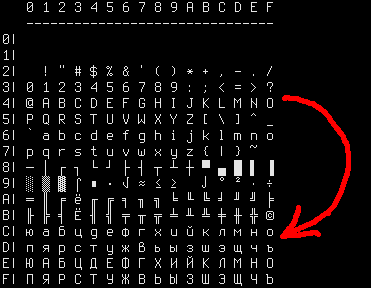
\includegraphics[width=0.5\textwidth]{fundamentals/koi8r.png}
\caption{KOI8-R table}
\end{figure}

Someone may notice that Cyrillic characters are allocated almost in the same sequence as Latin ones.
This leads to one important property: if all 8th bits in Cyrillic text encoded in KOI-8R are to be reset,
a text transforms into transliterated text with Latin characters in place of Cyrillic.
For example, Russian sentence:

\begin{framed}
\begin{quotation}
Мой дядя самых честных правил, Когда не в шутку занемог, Он уважать себя заставил, И лучше выдумать не мог.
\end{quotation}
\end{framed}

\dots if encoded in KOI-8R and then 8th bit stripped, transforms into:

\begin{framed}
\begin{quotation}
mOJ DQDQ SAMYH \^{}ESTNYH PRAWIL, kOGDA NE W [UTKU ZANEMOG, oN UWAVATX SEBQ ZASTAWIL, i LU\^{}[E WYDUMATX NE MOG.
\end{quotation}
\end{framed}

\dots perhaps this is not very appealing \ae{}sthetically, but this text is still readable to Russian language natives.

Hence, Cyrillic text encoded in KOI-8R, passed through an old 7-bit service will survive into transliterated, but still
readable text.

Stripping 8th bit is automatically transposes any character from the second half of
the (any) 8-bit \ac{ASCII} table to the first one, into the same place (take a look at red arrow right of table).
If the character has already been placed in the first half (i.e., it has been in standard 7-bit \ac{ASCII} table), it's not transposed.

Perhaps, transliterated text is still recoverable, if you'll add 8th bit to the characters which were seems
transliterated.

Drawback is obvious: Cyrillic characters allocated in KOI-8R table are not in the same sequence as
in Russian/Bulgarian/Ukrainian/etc. alphabet, and this isn't suitable for sorting, for example.

}\RU{\section{AND}

\subsection{Проверка того, находится ли значение на границе $2^n$}

Если нужно проверить, делится ли ваше значение на число вида 
$2^n$ (как 1024, 4096, итд.) без остатка,
вы можете использовать оператор \TT{\%} в \CCpp, но есть способ проще.
4096 это 0x1000, так что в нем всегда есть $4*3=12$ нулевых младших бит.

Что вам нужно, это просто:

\begin{lstlisting}[style=customc]
if (value&0xFFF)
{
	printf ("значение не делится на 0x1000 (или 4096)\n");
	printf ("кстати, остаток=%d\n", value&0xFFF);
}
else
	printf ("значение делится на 0x1000 (или 4096)\n");
\end{lstlisting}

Другими словами, это код проверяет, если здесь любой выставленный бит среди младших 12-и бит.
В качестве побочного эффекта, младщие 12 бит это всегда остаток от деления значения на 4096 (потому что деление на $2^n$
это лишь сдвиг вправо, и сдвинутые (или выброшенные) биты это биты остатка.

Та же история, если вам нужно проверить, является ли число четным или нет:

\begin{lstlisting}[style=customc]
if (value&1)
	// нечетное
else
	// четное
\end{lstlisting}

Это то же самое, как и деление на 2 и вычисление 1-битного остатка.

\subsection{Кирилличная кодировка KOI-8R}

Было время, когда 8-битная таблица \ac{ASCII} не поддерживалась некоторыми сервисами в Интернете, включая электронную почту.
Некоторые поддерживали, некоторые другие --- нет.

И это также было время, когда не-латинские системы письменности использовали вторую половину 8-битной таблицы ASCII
для размещения не-латинских символов.
Было несколько популярный кирилличных кодировок, но KOI-8R (придуманная Андреем ``ache'' Черновым)
в каком-то смысле уникальная, если сравнивать с другими.

% TODO invert arrow 
% TODO text latex form instead of png!
\begin{figure}[H]
\centering
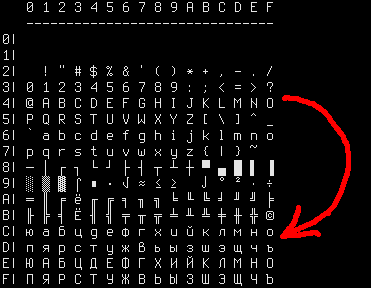
\includegraphics[width=0.5\textwidth]{fundamentals/koi8r.png}
\caption{KOI8-R table}
\end{figure}

Кое-кто может заметить, что кирилличные символы расположены почти в том же порядке, в котором и латинские.
Это приводит к важному свойству: если в кирилличном тексте закодированном в KOI-8R сбросить 8-й бит,
текст трансформируется в транслитерированный текст с латинскими символами на месте кирилличных.
Например, фраза на русском:

\begin{framed}
\begin{quotation}
Мой дядя самых честных правил, Когда не в шутку занемог, Он уважать себя заставил, И лучше выдумать не мог.
\end{quotation}
\end{framed}

\dots если закодирована в KOI-8R, и затем со сброшенным 8-м битом, трансформируется в:

\begin{framed}
\begin{quotation}
mOJ DQDQ SAMYH \^{}ESTNYH PRAWIL, kOGDA NE W [UTKU ZANEMOG, oN UWAVATX SEBQ ZASTAWIL, i LU\^{}[E WYDUMATX NE MOG.
\end{quotation}
\end{framed}

\dots конечно, выглядит это не очень эстетично, но этот текст читаем для тех, кто знает русский язык.

Следовательно, кирилличный текст закодированный в KOI-8R, пропущенный чере сервис поддерживающий только 7 бит,
выживет в виде транслитерированного, но читаемого текста.

Очистка 8-го бита автоматически транспонирует любой символ из второй половины (любой) 8-битной \ac{ASCII}-таблицы
в первую половину, в то же место (посмотрите на красную стрелку справа от таблицы).
Если символ уже расположен в первой половине (т.е., он находился в стандартной 7-битной \ac{ASCII}-таблице),
он не будет транспонироваться.

Вероятно, транслитерированный текст все еще можно восстановить, если вы прибавите 8-й бит к символам,
которые выглядят как транслитерированные.

Недостаток виден сразу: кирилличные символы расположенные в таблице KOI-8R расположены не в том порядке,
в каком они расположены в русском/болгарском/украинском/итд алфавите, и это не удобно для сортировки, например.

}

\EN{\section{AND and OR as subtraction and addition}

\subsection{ZX Spectrum ROM text strings}
\label{ZX Spectrum}

Those who once investigated ZX Spectrum \ac{ROM} internals, probably noticed that the last symbol of each text string is seemingly
absent.

\begin{figure}[H]
\centering
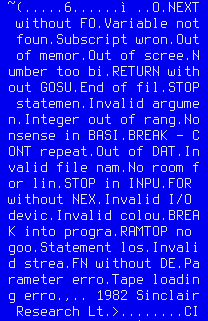
\includegraphics[width=0.3\textwidth]{fundamentals/zx_spectrum_ROM.png}
\caption{Part of ZX Spectrum ROM}
\end{figure}

There are present, in fact.

Here is excerpt of ZX Spectrum 128K ROM disassembled:

\lstinputlisting{fundamentals/ZX_Spectrum_ROM.lst}
( \url{http://www.matthew-wilson.net/spectrum/rom/128_ROM0.html} )

Last character has most significant bit set, which marks string end.
Presumably, it was done to save some space?
Old 8-bit computers has very tight environment.

Characters of all messages are always in standard 7-bit \ac{ASCII} table,
so it's guaranteed 8th bit is never used for characters.

To print such string, we must check \ac{MSB} of each byte, and if it's set, we must clear it, then print character,
and then stop.
Here is a C example:

\begin{lstlisting}[style=customc]
unsigned char hw[]=
{
	'H',
	'e',
	'l',
	'l',
	'o'|0x80
};

void print_string()
{
	for (int i=0; ;i++)
	{
		if (hw[i]&0x80) // check MSB
		{
			// clear MSB
			// (in other words, clear all, but leave 7 lower bits intact)
			printf ("%c", hw[i] & 0x7F);
			// stop
			break;
		};
		printf ("%c", hw[i]);
	};
};
\end{lstlisting}

Now what is interesting, since 8th bit is the most significant bit (in byte), we can check it, set it and remove it using
arithmetical operations instead of logical.

I can rewrite my C example:

\begin{lstlisting}[style=customc]
unsigned char hw[]=
{
	'H',
	'e',
	'l',
	'l',
	'o'+0x80
};

void print()
{
	for (int i=0; ;i++)
	{
		// hw[] must have 'unsigned char' type
		if (hw[i] >= 0x80) // check for MSB
		{
			printf ("%c", hw[i]-0x80); // clear MSB
			// stop
			break;
		};
		printf ("%c", hw[i]);
	};
};
\end{lstlisting}

By default, \IT{char} is signed type in C/C++, so to compare it with variable like 0x80 (which is negative ($-128$)
if treated as signed),
we must treat each character in text message as unsigned.

Now if 8th bit is set, the number is always larger or equal to 0x80.
If 8th bit is clear, the number is always smaller than 0x80.

Even more than that: if 8th bit is set, it can be cleared by subtracting 0x80, nothing else.
If it's not set beforehand, however, subtracting will destruct other bits.

Likewise, if 8th bit is clear, it's possible to set it by adding 0x80.
But if it's set beforehand, addition operation will destruct some other bits.

In fact, this is valid for any bit.
If the 4th bit is clear, you can set it just by adding 0x10: 0x100+0x10 = 0x110.
If the 4th bit is set, you can clear it by subtracting 0x10: 0x1234-0x10 = 0x1224.

It works, because carry isn't happened during addition/subtraction.
It will, however, happen, if the bit is already set there before addition, or absent before subtraction.

Likewise, addition/subtraction can be replaced using OR/AND operation if two conditions are met:
1) you want to add/subtract by a number in form of $2^n$;
2) this bit in source value is clear/set.

For example, addition of 0x20 is the same as ORing value with 0x20 under condition that this bit is clear before:
0x1204|0x20 = 0x1204+0x20 = 0x1224.

Subtraction of 0x20 is the same as ANDing value with ~0x20 (0x....FFDF), but if this bit is set before:
0x1234\&(\~{}0x20) = 0x1234\&0xFFDF = 0x1234-0x20 = 0x1214.

Again, it works because carry not happened when you add $2^n$ number and this bit isn't set before.

This property of boolean algebra is important, worth understanding and keeping it in mind.

}\RU{\section{\IT{И} и \IT{ИЛИ} как вычитание и сложение}

\subsection{Текстовые строки в \ac{ROM} ZX Spectrum}
\label{ZX Spectrum}

Те, кто пытался исследовать внутренности \ac{ROM} ZX Spectrum-а, вероятно, замечали,
что последний символ каждой текстовой строки как будто бы отсутствует.

\begin{figure}[H]
\centering
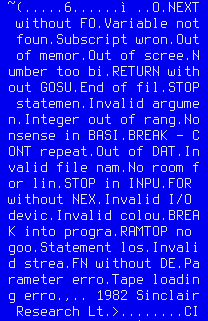
\includegraphics[width=0.3\textwidth]{fundamentals/zx_spectrum_ROM.png}
\caption{Часть \ac{ROM} ZX Spectrum}
\end{figure}

На самом деле, они присутствуют.

Вот фрагмент из дизассемблированного \ac{ROM} ZX Spectrum 128K:

\lstinputlisting{fundamentals/ZX_Spectrum_ROM.lst}
( \url{http://www.matthew-wilson.net/spectrum/rom/128_ROM0.html} )

Последний символ имеет выставленный старший бит, который означает конец строки.
Вероятно, так было сделано, чтобы сэкономить место?
В старых 8-битных компьютерах был сильный дефицит памяти.

Символы всех сообщений всегда находятся в стандартной 7-битной \ac{ASCII}-таблице, так что это гарантия,
что 8-й бит никогда не используется для символов.

Чтобы вывести такую строку, мы должны проверять \ac{MSB} каждого байта, и если он выставлен, мы должны его сбросить,
затем вывести символ, затем остановиться.
Вот пример на Си:

\begin{lstlisting}[style=customc]
unsigned char hw[]=
{
	'H',
	'e',
	'l',
	'l',
	'o'|0x80
};

void print_string()
{
	for (int i=0; ;i++)
	{
		if (hw[i]&0x80) // проверить MSB
		{
			// сбросить MSB
			// §(иными словами, сбросить всё, но оставить нетронутыми младшие 7 бит)§
			printf ("%c", hw[i] & 0x7F);
			// остановиться
			break;
		};
		printf ("%c", hw[i]);
	};
};
\end{lstlisting}

И вот что интересно, так как 8-й бит это самый старший бит (в байте), мы можем проверить его, выставить и сбросить
используя арифметические операции вместо логических.

Я могу переписать свой пример на Си:

\begin{lstlisting}[style=customc]
unsigned char hw[]=
{
	'H',
	'e',
	'l',
	'l',
	'o'+0x80
};

void print()
{
	for (int i=0; ;i++)
	{
		// hw[] должен иметь тип 'unsigned char'
		if (hw[i] >= 0x80) // проверить MSB
		{
			printf ("%c", hw[i]-0x80); // сбросить MSB
			// останов
			break;
		};
		printf ("%c", hw[i]);
	};
};
\end{lstlisting}

\IT{char} по умолчанию это знаковый тип в \CCpp, так что, чтобы сравнивать его с переменной вроде 0x80 (которая отрицательная
($-128$),
если считается за знаковую),
мы должны считать каждый символ сообщения как беззнаковый.

Теперь, если 8-й бит выставлен, число всегда больше или равно 0x80.
Если 8-й бит сброшен, число всегда меньше 0x80.

И даже более того: если 8-й бит выставлен, его можно сбросить вычитанием 0x80, и ничего больше.
Если он уже сброшен, впрочем, операция вычитания уничтожит другие биты.

Точно также, если 8-й бит сброшен, можно его выставить прибавлением 0x80.
Но если он уже выставлен, операция сложения уничтожит остальные биты.

На самом деле, это справедливо для любого бита.
Если 4-й бит сброшен, вы можете выставить его просто прибавлением 0x10: 0x100+0x10 = 0x110.
Если 4-й бит выставлен, вы можете его сбросить вычитанием 0x10: 0x1234-0x10 = 0x1224.

Это работает, потому что перенос не случается во время сложения/вычитания.
Хотя, он случится если бит уже выставлен перед сложением или сброшен перед вычитанием.

Точно также, сложение/вычитание можно заменить на операции \IT{ИЛИ/И} если справедливы два условия:
1) вы хотите прибавить/вычесть число вида $2^n$;
2) бит в исходном значение сброшен/выставлен.

Например, прибавление 0x20 это то же что и применение \IT{ИЛИ} со значением 0x20 с условием что этот бит был сброшен перед
этим:
0x1204|0x20 = 0x1204+0x20 = 0x1224.

Вычитание 0x20 это то же что и применение \IT{И} со значением ~0x20 (0x....FFDF), но если этот бит был выставлен до этого:
0x1234\&(\~{}0x20) = 0x1234\&0xFFDF = 0x1234-0x20 = 0x1214.

Опять же, это работает потому что перенос не случается если вы прибавляете число вида $2^n$ и этот бит до этого сброшен.

Это важное свойство булевой алгербы, его стоит понимать и помнить о нем.

}

\EN{\section{XOR (exclusive OR)}
\label{XOR_property}

\XOR is widely used when one needs just to flip specific bit(s).
Indeed, the \XOR operation applied with 1 effectively inverts a bit:

\begin{center}
\begin{tabular}{ | l | l | l | }
\hline
\HeaderColor \MLinputA & \HeaderColor \MLinputB & \HeaderColor \MLoutput \\
\hline
0 & 0 & 0 \\
\hline
{\color{red} 0} & {\color{red} 1} & {\color{red} 1} \\
\hline
{\color{red} 1} & {\color{red} 0} & {\color{red} 1} \\
\hline
1 & 1 & 0 \\
\hline
\end{tabular}
\end{center}


And vice-versa, the \XOR operation applied with 0 does nothing, i.e., it's an idle operation.
This is a very important property of the \XOR operation and it's highly recommended to memorize it.



\subsection{Everyday speech}

XOR operation present in common everyday speech.
When someone asks ``please buy apples or bananas'',
this usually means ``buy the first object or the second, but not both''---this is exactly exclusive OR,
because logical OR would mean ``both objects are also fine''.

Some people suggest ``and/or'' should be used in everyday speech to make emphasis that logical OR is used instead of
exclusive OR: \url{https://en.wikipedia.org/wiki/And/or}.

\subsection{Encryption}

XOR is heavily used in both amateur (\ref{simple_XOR_encryption}) and \IT{real} encryption (at least in \IT{Feistel network}).

XOR is very useful here because:
$cipher\_text = plain\_text \oplus key$ and then:
$(plain\_text \oplus key) \oplus key = plain\_text$.

\subsection{\ac{RAID}4}
\index{RAID4}

\ac{RAID}4 offers a very simple method to to protect hard disks.
For example, there are several disks ($D_1$, $D_2$, $D_3$, etc.) and one parity disk ($P$).
Each bit/byte written to parity disk is calculated and written on-fly:

\begin{equation} \label{eq:RAID4}
P = D_1 \oplus D_2 \oplus D_3
\end{equation}

If any of disks is failed, for example, $D_2$, it's restored using the very same way:

\begin{equation}
D_2 = D_1 \oplus P \oplus D_3
\end{equation}

If parity disk failed, it is restored using \ref{eq:RAID4} way.
If two of any disks are failed, then it wouldn't be possible to restore both.

\ac{RAID}5 is more advanced, but this XOR property is still exploited there.

That's why \ac{RAID} controllers has hardware ``XOR accelerators'' helping to XOR large chunks of written data on-fly.
When computers get faster and faster, it now can be done at software level, using \ac{SIMD}.

\subsection{XOR swap algorithm}

Hard to believe, but this code swaps values in \EAX and \EBX without aid of any other additional register or memory cell:

\begin{lstlisting}[style=customasmx86]
xor eax, ebx
xor ebx, eax
xor eax, ebx
\end{lstlisting}

Let's find out, how it works.
First, we will rewrite it to step aside from x86 assembly language:

\begin{lstlisting}
X = X XOR Y
Y = Y XOR X
X = X XOR Y
\end{lstlisting}

What X and Y has at each step?
Just keep in mind the simple rule: $(X \oplus Y) \oplus Y = X$ for any values of X and Y.

Let's see,
$X$ after 1st step has $X \oplus Y$;
$Y$ after 2nd step has $Y \oplus (X \oplus Y) = X$;
$X$ after 3rd step has $(X \oplus Y) \oplus X = Y$.

Hard to say if anyone should use this trick, but it servers as a good demonstration example of XOR properties.

Wikipedia article (\url{https://en.wikipedia.org/wiki/XOR_swap_algorithm}) has also yet another explanation:
addition and subtraction operations can be used instead of XOR:

\begin{lstlisting}
X = X + Y
Y = X - Y
X = X - Y
\end{lstlisting}

Let's see:
$X$ after 1st step has $X+Y$;
$Y$ after 2nd step has $X+Y-Y=X$;
$X$ after 3rd step has $X+Y-X=Y$.

\subsection{XOR linked list}
\index{Doubly linked list}

Doubly linked list is a list in which each element has link to the previous element and to the next one.
Hence, it's very easy to traverse list backwards or forward.
\TT{std::list} in C++ implements doubly linked list which also is examined in this book: \ref{std_list}.

So each element has two pointers.
Is it possible, perhaps in environment of small \ac{RAM} footprint, to preserve all functionality with one pointer instead of two?
Yes, if it a value of $prev \oplus next$ will be stored in this memory cell, which is usually called ``link''.

Maybe, we could say that address to the previous element is ``encrypted'' using address of next element and otherwise:
next element address is ``encrypted'' using previous element address.

When we traverse this list forward, we always know address of the previous element, so we can ``decrypt'' this field and get 
address of the next element.
Likewise, it's possible to traverse this list backwards, ``decrypting'' this field using next element's address.

But it's not possible to find address of previous or next element of some specific element without
knowing address of the first one.

Couple of things to complete this solution: first element will have address of next element without any XOR-ing,
last element will have address of previous element without any XOR-ing.

Now let's sum it up. This is example of doubly linked list of 5 elements.
$A_x$ is address of element.

\begin{center}
\begin{tabular}{ | l | l | }
	\hline
	\HeaderColor address & \HeaderColor \IT{link} field contents \\
	\hline
	$A_0$ & $A_1$ \\
	\hline
	$A_1$ & $A_0 \oplus A_2$ \\
	\hline
	$A_2$ & $A_1 \oplus A_3$ \\
	\hline
	$A_3$ & $A_2 \oplus A_4$ \\
	\hline
	$A_4$ & $A_3$ \\
	\hline
\end{tabular}
\end{center}

And again, hard to say if anyone should use this tricky hacks, but this is also a good demonstration of XOR properties.
As with XOR swap algorithm, Wikipedia article about it also offers way to use addition or subtraction instead of XOR:
\url{https://en.wikipedia.org/wiki/XOR_linked_list}.

\subsection{By the way}

The usual \IT{OR} also sometimes called \IT{inclusive OR} (or even \IT{IOR}), as opposed to \IT{exclusive OR}.

}\RU{\section{XOR (исключающее \IT{ИЛИ})}
\label{XOR_property}

\XOR (исключающее ИЛИ) часто используется для того чтобы поменять какой-то бит(ы) на противоположный.
Действительно, операция \XOR с 1 на самом деле просто инвертирует бит:

\begin{center}
\begin{tabular}{ | l | l | l | }
\hline
\HeaderColor \MLinputA & \HeaderColor \MLinputB & \HeaderColor \MLoutput \\
\hline
0 & 0 & 0 \\
\hline
{\color{red} 0} & {\color{red} 1} & {\color{red} 1} \\
\hline
{\color{red} 1} & {\color{red} 0} & {\color{red} 1} \\
\hline
1 & 1 & 0 \\
\hline
\end{tabular}
\end{center}


И наоборот, операция \XOR с 0 ничего не делает, т.е. это холостая операция.
Это очень важное свойство операции \XOR и очень важно помнить его.


\subsection{Бытовая речь}

Оперция XOR присутствует в обычной бытовой речи.
Когда кто-то просит ``пожалуйста, купи яблок или бананов'',
это обычно означает ``купи первый объект, или второй, но не оба'' --- это и есть исключающее ИЛИ,
потому что логическое ИЛИ означало бы ``оба объекта тоже сгодятся''.

Некоторые люди предлагают использовать в речи ``и/или'', чтобы подчеркнуть тот факт, что используется именно логическое ИЛИ
вместо исключающего ИЛИ: \url{https://en.wikipedia.org/wiki/And/or}.

\subsection{Шифрование}

Исключающее ИЛИ много используется как в любительской криптографии (\ref{simple_XOR_encryption}), так и в \IT{настоящей}
(как минимум в \IT{сети Фестеля}).

Эта операция очень удобна потому что:
\IT{шифрованный\_текст = исходный\_текст $\oplus$ ключ} и затем:
\IT{(исходный\_текст $\oplus$ ключ) $\oplus$ ключ = исходный\_текст}.

\subsection{\ac{RAID}4}
\index{RAID4}

\ac{RAID}4 предлагает очень простой метод защиты жестких дисков.
Например, есть несколько дисков ($D_1$, $D_2$, $D_3$, итд.) и один диск чётности (\IT{parity disk}) ($P$).
Каждый бит/байт записываемый на диск чётности вычисляется на лету:

\begin{equation} \label{eq:RAID4}
P = D_1 \oplus D_2 \oplus D_3
\end{equation}

Если один из дисков испортился, например, $D_2$, он восстанавливается точно также:

\begin{equation}
D_2 = D_1 \oplus P \oplus D_3
\end{equation}

Если диск чётности испортился, он восстанавливается так же: \ref{eq:RAID4}.
Если два любых диска испортились, тогда уже не получится восстановить оба.

\ac{RAID}5 развился далее, но эта особенность исключающего ИЛИ используется и там.

Вот почему в контроллерах \ac{RAID} были ``XOR-акселлераторы'', они помогали XOR-ить большие объемы данных
на лету, перед записью на диски.
Когда компьютеры стали быстрее, стало возможным делать это же программно, используя \ac{SIMD}.

\subsection{Алгоритм обмена значений при помощи исключающего ИЛИ}

Трудно поверить, но этот код меняет значения в \EAX и \EBX без помощи вспомогательного регистра или ячейки памяти:

\begin{lstlisting}[style=customasmx86]
xor eax, ebx
xor ebx, eax
xor eax, ebx
\end{lstlisting}

Посмотрим, как это работает.
Для начала, мы перепишем этот код, чтобы отойти от ассемблера x86:

\begin{lstlisting}
X = X XOR Y
Y = Y XOR X
X = X XOR Y
\end{lstlisting}

Что содержат X и Y на каждом шаге?
Просто держите в памяти простое правило: $(X \oplus Y) \oplus Y = X$ для любых значений X и Y.

Посмотрим,
$X$ после первого шага это $X \oplus Y$;
$Y$ после второго шага это $Y \oplus (X \oplus Y) = X$;
$X$ после третьего шага это $(X \oplus Y) \oplus X = Y$.

Трудно сказать, стоит ли использовать этот трюк, но он служит неплохой демонстрацией свойств исключающего ИЛИ.

В статье Wikipedia (\url{https://en.wikipedia.org/wiki/XOR_swap_algorithm}) есть еще такое объяснение:
можно использовать сложение и вычитание вместо исключающего ИЛИ:

\begin{lstlisting}
X = X + Y
Y = X - Y
X = X - Y
\end{lstlisting}

Посмотрим:
$X$ после первого шага это $X+Y$;
$Y$ после второго шага это $X+Y-Y=X$;
$X$ после третьего шага это $X+Y-X=Y$.

\subsection{Список связанный при помощи XOR}
\index{Doubly linked list}

Двусвязный список это список, в котором каждый элемент имеет ссылку на предыдущий элемент и на следующий.
Следовательно, легко перечислять элементы и вперед и назад.
\TT{std::list} в Си++ реализует двусвязный список, и он рассматривается в этой книге: \ref{std_list}.

Так что каждый элемент имеет два указателя.
Возможно ли, вероятно, в среде где нужно экономить \ac{RAM}, сохранить всю функциональность используя один указатель
вместо двух?
Да, если будем хранить значение $предыдущий \oplus следующий$ в ячейке, которую обычно называют ``link''.

Можно быть, мы можем сказать, что адрес предыдущего элемента ``зашифрован'' используя адрес следующего элемента и наоборот:
адрес следующего элемента ``зашифрован'' используя адрес предыдущего элемента.

Когда мы проходим по списку вперед, мы всегда знаем адрес предыдущего элемента, так что мы можем ``расшифровать'' это поле
и получить адрес следующего элемента.
Точно также, мы можем пройти по списку назад, ``дешифруя'' это поле используя адрес следующего элемента.

Но невозможно найти адрес предыдущего или следующего элемента определенного элемента без знания адреса первого элемента.

Еще кое-что: первый элемент будем иметь адрес следующего элемента без ничего,
последний элемент будет иметь адрес предыдущего элемента без ничего.

Подведем итоги. Это пример двусвязного списка из 5-и элементов.
$A_x$ это адрес элемента.

\begin{center}
\begin{tabular}{ | l | l | }
	\hline
	\HeaderColor адрес & \HeaderColor содержимое поля \IT{link} \\
	\hline
	$A_0$ & $A_1$ \\
	\hline
	$A_1$ & $A_0 \oplus A_2$ \\
	\hline
	$A_2$ & $A_1 \oplus A_3$ \\
	\hline
	$A_3$ & $A_2 \oplus A_4$ \\
	\hline
	$A_4$ & $A_3$ \\
	\hline
\end{tabular}
\end{center}

И снова, трудно сказать, нужно ли использовать эти хаки, но это также хорошая демонстрация особенностей исключающего ИЛИ.
Как и с алгоритмом обмена значений при помощи исключающего ИЛИ, в статье Wikipedia есть также предложение использовать
сложение или вычитание вместо исключающего ИЛИ:
\url{https://en.wikipedia.org/wiki/XOR_linked_list}.

\subsection{Кстати}

Обычное \IT{ИЛИ} иногда называют \IT{включающее ИЛИ} (\IT{inclusive OR}, или даже \IT{IOR}),
чтобы противопоставить его \IT{исключающему ИЛИ}.

}

\EN{\subsection{AND/OR/XOR as MOV}

\INS{OR reg, 0xFFFFFFFF} sets all bits to 1, hence, no matter what has been in register before, it will be set to $-1$.
\INS{OR reg, -1} is shorter than \INS{MOV reg, -1}, so MSVC uses OR instead the latter,
for example: \myref{using_OR_instead_of_MOV}.

Likewise, \INS{AND reg, 0} always resets all bits, hence, it acts like \INS{MOV reg, 0}.

\INS{XOR reg, reg}, no matter what has been in register beforehand, resets all bits, and also acts like \INS{MOV reg, 0}.

}
\ES{
\subsection{AND/OR/XOR como MOV}

\INS{OR reg, 0xFFFFFFFF} establece todos los bits a 1, por lo tanto, no importa lo que estaba antes en el registro, este ser\'a establecido a $-1$.
\INS{OR reg, -1} es m\'as corto que \INS{MOV reg, -1}, as\'í que MSVC usa el OR en vez del MOV.

por ejemplo \myref{using_OR_instead_of_MOV}.

As\'i, \INS{AND reg, 0} siempre resetea todos los bits, por lo tanto, act\'ua como un \INS{MOV reg, 0}.

\INS{XOR reg, reg}, resetea todos los bits, sin importar lo que estuviese antes en el registro, y tambi\'en es quivalente a un \INS{MOV reg, 0}.
}
\RU{\subsection{AND/OR/XOR как MOV}

Инструкция \INS{OR reg, 0xFFFFFFFF} выставляет все биты в 1, следовательно, не важно что было в регистре перед этим,
его значение будет выставлено в $-1$.
Инструкция \INS{OR reg, -1} короче, чем \INS{MOV reg, -1}, так что MSVC использует OR вместо последней,
например: \myref{using_OR_instead_of_MOV}.

Точно также, \INS{AND reg, 0} всегда сбрасывает все биты, следовательно, работает как \INS{MOV reg, 0}.

\INS{XOR reg, reg}, не важно что было в регистре перед этим, сбрасывает все биты, и также работает как \INS{MOV reg, 0}.

}

\EN{\section{Population count}
\label{POPCNT}

\INS{POPCNT} instruction is population count (\ac{AKA} Hamming weight).
It just counts number of bits set in an input value.

As a side effect, \INS{POPCNT} instruction (or operation) can be used to determine, if the value has $2^n$ form.
Since, $2^n$ number always has just one single bit, \INS{POPCNT}'s result will always be just 1.

\myindex{base64scanner}
For example, I once wrote a base64 strings scanner for hunting something interesting in binary files\footnote{\url{https://github.com/dennis714/base64scanner}}.
And there is a lot of garbage and false positives, so I add an option to filter out data blocks which has size of $2^n$ bytes
(i.e., 256 bytes, 512, 1024, etc.).
The size of block is checked just like this:

\begin{lstlisting}[style=customc]
if (popcnt(size)==1)
	// OK
...
\end{lstlisting}

The instruction is also known as \q{\ac{NSA} instruction} due to rumors:

\begin{framed}
\begin{quotation}
  This branch of cryptography is fast-paced and very politically charged.
  Most designs are secret; a majority of military encryptions systems in use today are 
  based on LFSRs. 
  In fact, most Cray computers (Cray 1, Cray X-MP, Cray Y-MP) have a rather curious 
  instruction generally known as “population count.” It counts the 1 bits in a register 
  and can be used both to efficiently calculate the Hamming distance between two binary 
  words and to implement a vectorized version of a LFSR. I’ve heard this called the canonical 
  NSA instruction, demanded by almost all computer contracts.
\end{quotation}
\end{framed}
\InSqBrackets{\Schneier{}}

}\RU{\section{Подсчет бит}
\label{POPCNT}

Инструкция \INS{POPCNT} (\IT{population count}) служит для подсчета бит во входном значении (\ac{AKA} расстояние Хэмминга).

В качестве побочного эффекта, инструкция \INS{POPCNT} (или операция) может использоваться, чтобы узнать,
имеет ли значение вид $2^n$.
Так как числа $2^n$ всегда имеют только один выставленный бит, результат \INS{POPCNT} всегда будет просто 1.

\myindex{base64scanner}
Например, я однажды написал сканер для поиска base64-строк в бинарных файлах\footnote{\url{https://github.com/dennis714/base64scanner}}.
И есть много мусора и ложных срабатываний, так что я добавил опцию для фильтрования блоков данных, размер которых $2^n$ байт
(т.е., 256 байт, 512, 1024, итд.).
Размер блока проверяется так:

\begin{lstlisting}[style=customc]
if (popcnt(size)==1)
	// OK
...
\end{lstlisting}

Инструкция также известна как \q{инструкция \ac{NSA}} из-за слухов:

\begin{framed}
\begin{quotation}
  This branch of cryptography is fast-paced and very politically charged.
  Most designs are secret; a majority of military encryptions systems in use today are 
  based on LFSRs. 
  In fact, most Cray computers (Cray 1, Cray X-MP, Cray Y-MP) have a rather curious 
  instruction generally known as “population count.” It counts the 1 bits in a register 
  and can be used both to efficiently calculate the Hamming distance between two binary 
  words and to implement a vectorized version of a LFSR. I’ve heard this called the canonical 
  NSA instruction, demanded by almost all computer contracts.
\end{quotation}
\end{framed}
\InSqBrackets{\Schneier{}}

}

\EN{\section{Endianness}
\label{sec:endianness}

The endianness is a way of representing values in memory.

\subsection{Big-endian}

The \TT{0x12345678} value is represented in memory as:

\begin{center}
\begin{tabular}{ | l | l | }
\hline
\HeaderColor address in memory & \HeaderColor byte value \\
\hline
+0 & 0x12 \\
\hline
+1 & 0x34 \\
\hline
+2 & 0x56 \\
\hline
+3 & 0x78 \\
\hline
\end{tabular}
\end{center}

Big-endian CPUs include Motorola 68k, IBM POWER.

\subsection{Little-endian}

The \TT{0x12345678} value is represented in memory as:

\begin{center}
\begin{tabular}{ | l | l | }
\hline
\HeaderColor address in memory & \HeaderColor byte value \\
\hline
+0 & 0x78 \\
\hline
+1 & 0x56 \\
\hline
+2 & 0x34 \\
\hline
+3 & 0x12 \\
\hline
\end{tabular}
\end{center}

Little-endian CPUs include Intel x86.

\subsection{\Example}

Let's take big-endian MIPS Linux installed and ready in QEMU
\footnote{Available for download here: \url{http://go.yurichev.com/17008}}.

And let's compile this simple example:

\begin{lstlisting}[style=customc]
#include <stdio.h>

int main()
{
	int v, i;

	v=123;

	printf ("%02X %02X %02X %02X\n", 
		*(char*)&v,
		*(((char*)&v)+1),
		*(((char*)&v)+2),
		*(((char*)&v)+3));
};
\end{lstlisting}

After running it we get:

\begin{lstlisting}
root@debian-mips:~# ./a.out 
00 00 00 7B
\end{lstlisting}

That is it.
0x7B is 123 in decimal.
In little-endian architectures, 7B is the first byte (you can check on x86 or x86-64), 
but here it is the last one, because the highest byte goes first.

That's why there are separate Linux distributions for MIPS
(\q{mips} (big-endian) and \q{mipsel} (little-endian)).
It is impossible for a binary compiled for one endianness to work on an \ac{OS} with different endianness. 

There is another example of MIPS big-endiannes in this book: \myref{MIPS_structure_big_endian}.

\subsection{Bi-endian}

CPUs that may switch between endianness are ARM, PowerPC, SPARC, MIPS, \ac{IA64}, etc.

\subsection{Converting data}

\myindex{x86!\Instructions!BSWAP}
The \TT{BSWAP} instruction can be used for conversion.

\myindex{TCP/IP}
TCP/IP network data packets use the big-endian conventions, so that is why a program working on a little-endian architecture
has to convert the values.
The \TT{htonl()} and \TT{htons()} functions are usually used.

In TCP/IP, big-endian is also called \q{network byte order}, while byte order on the computer \q{host byte order}.
\q{host byte order} is little-endian on Intel x86 and other little-endian architectures,
but it is big-endian on IBM POWER, so \TT{htonl()} and \TT{htons()} don't shuffle any bytes on the latter.

}\ES{\section{Endianness}
\label{sec:endianness}

Endianness es una forma de representar valores en la memoria.

\subsection{Big-endian}

El valor \TT{0x12345678} es representado en la memoria como:

\begin{center}
\begin{tabular}{ | l | l | }
\hline
\HeaderColor direcci\'on en memoria & \HeaderColor valor del byte \\
\hline
+0 & 0x12 \\
\hline
+1 & 0x34 \\
\hline
+2 & 0x56 \\
\hline
+3 & 0x78 \\
\hline
\end{tabular}
\end{center}

Entre los CPU big-endian se encuentran Motorola 68k, IBM POWER.

\subsection{Little-endian}

El valor \TT{0x12345678} es representado en la memoria como:

\begin{center}
\begin{tabular}{ | l | l | }
\hline
\HeaderColor Direcci\'on en memoria & \HeaderColor valor del byte \\
\hline
+0 & 0x78 \\
\hline
+1 & 0x56 \\
\hline
+2 & 0x34 \\
\hline
+3 & 0x12 \\
\hline
\end{tabular}
\end{center}

Entre los CPU little-endian tenemos el Intel x86.

\subsection{\Example}

Tomemos el MIPS big-endian para Linux instalado y listo en QEMU
\footnote{Disponible para descargar aqu\'i: \url{http://go.yurichev.com/17008}%}.

Y compilemos este ejemplo sencillo:

\begin{lstlisting}[style=customc]
#include <stdio.h>

int main()
{
	int v, i;

	v=123;

	printf ("%02X %02X %02X %02X\n", 
		*(char*)&v,
		*(((char*)&v)+1),
		*(((char*)&v)+2),
		*(((char*)&v)+3));
};
\end{lstlisting}

Despu\'es de correrlo obtenemos:

\begin{lstlisting}
root@debian-mips:~# ./a.out 
00 00 00 7B
\end{lstlisting}

Eso es todo.
0x7B es 123 en decimal.
En las arquitecturas little-endian, 7B es el primer byte (puedes checarlo en x86 o x86-64),
pero aqu\'i es el \'ultimo, porque el byte m\'as alto va primero.

Por eso hay distribuciones separadas de Linux para MIPS
(\q{mips} (big-endian) \ESph{} \q{mipsel} (little-endian)).
Es imposible que un binario compilado para un endianness trabaje en un SO con diferente endianness.

En este libro hay otro ejemplo de big-endianness en MIPS: \myref{MIPS_structure_big_endian}.

\subsection{Bi-endian\RU{ (переключаемый порядок)}}

CPUs que puede cambiar entre endianness son ARM, PowerPC, SPARC, MIPS, \ac{IA64}, etc.

\subsection{Convirtiendo datos}

\myindex{x86!\Instructions!BSWAP}
La instrucci\'on \TT{BSWAP} puede ser utilizada para conversiones.

\myindex{TCP/IP}
Los paquetes de datos en redes TCP/IP utilizan convenciones big-endian, por eso un programa corriendo en una arquitectura
little-endian tiene que convertir los valores.

Las funciones \TT{htonl()} \ESph{} \TT{htons()} son usadas generalmente.

En TCP/IP, big-endian tambi\'en es llamado \q{orden de bytes de red},
mientras que el orden de bytes en la computadora se conoce como \q{orden de bytes de host}.
\q{orden de bytes de host} es little-endian en Intel x86 y otras arquitecturas little-endian,
pero es big-endian en IBM POWER, asi que \TT{htonl()} y \TT{htons()} no cambian el orden de los bytes
en \'esta \'ultima.

}\RU{\section{Endianness (порядок байт)}
\label{sec:endianness}

Endianness (порядок байт) это способ представления чисел в памяти.

\subsection{Big-endian (от старшего к младшему)}

Число \TT{0x12345678} представляется в памяти так:

\begin{center}
\begin{tabular}{ | l | l | }
\hline
\HeaderColor адрес в памяти & \HeaderColor значение байта \\
\hline
+0 & 0x12 \\
\hline
+1 & 0x34 \\
\hline
+2 & 0x56 \\
\hline
+3 & 0x78 \\
\hline
\end{tabular}
\end{center}

CPU с таким порядком включают в себя Motorola 68k, IBM POWER.

\subsection{Little-endian (от младшего к старшему)}

Число \TT{0x12345678} представляется в памяти так:

\begin{center}
\begin{tabular}{ | l | l | }
\hline
\HeaderColor адрес в памяти & \HeaderColor значение байта \\
\hline
+0 & 0x78 \\
\hline
+1 & 0x56 \\
\hline
+2 & 0x34 \\
\hline
+3 & 0x12 \\
\hline
\end{tabular}
\end{center}

CPU с таким порядком байт включают в себя Intel x86.

\subsection{\Example}

Возьмем big-endian Linux для MIPS заинсталированный в QEMU
\footnote{Доступен для скачивания здесь: \url{http://go.yurichev.com/17008}}.

И скомпилируем этот простой пример:

\begin{lstlisting}[style=customc]
#include <stdio.h>

int main()
{
	int v, i;

	v=123;

	printf ("%02X %02X %02X %02X\n", 
		*(char*)&v,
		*(((char*)&v)+1),
		*(((char*)&v)+2),
		*(((char*)&v)+3));
};
\end{lstlisting}

И запустим его:

\begin{lstlisting}
root@debian-mips:~# ./a.out 
00 00 00 7B
\end{lstlisting}

Это оно и есть.
0x7B это 123 в десятичном виде.
В little-endian-архитектуре, 7B это первый байт (вы можете это проверить в x86 или x86-64),
но здесь он последний, потому что старший байт идет первым.

Вот почему имеются разные дистрибутивы Linux для MIPS
(\q{mips} (big-endian) и \q{mipsel} (little-endian)).
Программа скомпилированная для одного соглашения об endiannes, не сможет работать в OS использующей
другое соглашение.

Еще один пример связанный с big-endian в MIPS в этой книге: \myref{MIPS_structure_big_endian}.

\subsection{Bi-endian (переключаемый порядок)}

CPU поддерживающие оба порядка, и его можно переключать, включают в себя ARM, PowerPC, SPARC, MIPS, \ac{IA64}, итд.

\subsection{Конвертирование}

\myindex{x86!\Instructions!BSWAP}
Инструкция \TT{BSWAP} может использоваться для конвертирования.

\myindex{TCP/IP}
Сетевые пакеты TCP/IP используют соглашение big-endian, вот почему программа, работающая на little-endian архитектуре
должна конвертировать значения.

Обычно, используются функции \TT{htonl()} и \TT{htons()}.

Порядок байт big-endian в среде TCP/IP также называется, \q{network byte order},
а порядок байт на компьютере \q{host byte order}.
На архитектуре Intel x86, и других little-endian архитектурах, \q{host byte order} это little-endian, 
а вот на IBM POWER это может быть big-endian, так что на последней, 
\TT{htonl()} и \TT{htons()} не меняют порядок байт.

}

\EN{\section{Memory}

There are 3 main types of memory:

\begin{itemize}
\item
Global memory \ac{AKA} \q{static memory allocation}.
No need to allocate explicitly, the allocation is performed just by declaring variables/arrays 
globally.
These are global variables, residing in the data or constant segments.
They are available globally (hence, considered as an \gls{anti-pattern}).
Not convenient for buffers/arrays, because they must have a fixed size.
Buffer overflows that occur here usually overwrite variables or buffers residing next to them in memory.
There's an example in this book: \myref{scanf_global_variable}.

\item
Stack \ac{AKA} \q{allocate on stack}.
The allocation is performed just by declaring variables/arrays locally in the function.
These are usually local variables for the function.
Sometimes these local variable are also available to descending functions 
(to \gls{callee} functions, if caller passes a pointer to a variable to the \gls{callee} to be executed).
Allocation and deallocation are very fast, it just \ac{SP} needs to be shifted.
\myindex{\CStandardLibrary!alloca()}

But they're also not convenient for buffers/arrays, because the buffer size has to be fixed,
unless \TT{alloca()} (\myref{alloca}) (or a variable-length array) is used.
Buffer overflows usually overwrite important stack structures: \myref{subsec:bufferoverflow}.

\myindex{\CStandardLibrary!malloc()}
\myindex{\CStandardLibrary!free()}
\item
Heap \ac{AKA} \q{dynamic memory allocation}.
Allocation/deallocation is performed by calling \\
\TT{malloc()/free()} or \TT{new/delete} in \Cpp.
This is the most convenient method: the block size may be set at runtime.
\myindex{\CStandardLibrary!realloc()}

Resizing is possible (using \TT{realloc()}), but can be slow.
This is the slowest way to allocate memory: 
the memory allocator must support and update all control structures while
allocating and deallocating.
Buffer overflows usually overwrite these structures.
Heap allocations are also source of memory leak problems: each memory block has to be deallocated
explicitly, but one may forget about it, or do it incorrectly.
\myindex{\CStandardLibrary!free()}

Another problem is the \q{use after free}---using a memory block after \TT{free()} has been called on it,
which is very dangerous.

Example in this book: \myref{struct_malloc_example}.

\end{itemize}
}\ES{% TODO probably needs to be resynchronized with EN version
\section{Memoria}

Existen 3 tipos principales de memoria:

\begin{itemize}
\item
Memoria global \ac{AKA} \q{asignaci\'on est\'atica de memoria}.
No hay necesidad de asignarla expl\'icitamente, la asignaci\'on es realizada al declarar
variables/arreglos globales.
Estas variables globales residen en los segmentos de datos o de constantes.
Est\'an disponibles globalmente (por lo tanto, se consideran un anti-patr\'on).
No son convenientes para buffers/arreglos porque deben tener un tama\~no fijo.
Los desbordamientos de buffer que occurren aqu\'i usualmente sobreescriben variables o buffers que residen
junto a ellos en memoria.
En este libro hay un ejemplo: \myref{scanf_global_variable}.

\item
Pila \ac{AKA} \q{asignaci\'on en pila}.
La asignaci\'on se realiza al declarar variables/arreglos dentro de una funci\'on.
Son usualmente variables locales a la funci\'on.
Algunas veces estas variables locales tambi\'en estan disponibles para funciones descendientes
(funciones llamadas, si aquel que la llama le pasa un apuntador a una de sus variables).
La asignaci\'on y desasignaci\'on son muy r\'apidas, s\'olo necesita que \ac{SP} sea ajustado.
\myindex{\CStandardLibrary!alloca()}
\ESph{}
Los desbordamientos de buffer suelen reescribir estructuras importantes en la pila: \myref{subsec:bufferoverflow}.

\myindex{\CStandardLibrary!malloc()}
\myindex{\CStandardLibrary!free()}
\item
Heap \ac{AKA} \q{asignaci\'on din\'amica de memoria}.
La asignaci\'on/desasignaci\'on es realizada llamando a \\
\TT{malloc()/free()} \ESph{} \TT{new/delete} \ESph{} \Cpp.
\'Este es el m\'etodo m\'as conveniente: el tama\~no del bloque puede establecerse en tiempo de ejecuci\'on.
\myindex{\CStandardLibrary!realloc()}
Cambiar el tama\~no es posible (usando \TT{realloc()}), pero puede ser lento.
\'Esta es la forma m\'as lenta de asignar memoria:
el asignador de memoria debe suportar y actualizar todas las estructuras de control
mientras se asigna y desasigna.
Los desbordamientos de buffer suelen sobreescribir estas estructuras.
Las asiganciones en el heap tambi\'en son el origen de problemas de fuga de memoria: cada bloque de memoria tiene
que ser desasgnado expl\'icitamente, pero uno puede olvidarse de ello, o hacerlo de manera incorrecta.
\myindex{\CStandardLibrary!free()}
Otro problema es el \q{uso despu\'es de la liberaci\'on}---usar un bloque de memoria despu\'es
de que \TT{free()} ha sido llamado en \'el, lo cual es muy peligroso.
Un ejemplo en este libro:
\myref{struct_malloc_example}.

\end{itemize}
}\RU{\section{Память}

Есть три основных типа памяти:

\begin{itemize}
\item
Глобальная память \ac{AKA} \q{static memory allocation}.
Нет нужды явно выделять, выделение происходит просто при объявлении переменных/массивов 
глобально.
Это глобальные переменные расположенные в сегменте данных или констант.
Доступны глобально (поэтому считаются \glslink{anti-pattern}{анти-паттерном}).
Не удобны для буферов/массивов, потому что должны иметь фиксированный размер.
Переполнения буфера, случающиеся здесь, обычно перезаписывают переменные или буферы
расположенные рядом в памяти.
Пример в этой книге: \myref{scanf_global_variable}.

\item
Стек \ac{AKA} \q{allocate on stack}, \q{выделить память в/на стеке}.
Выделение происходит просто при объявлении переменных/массивов локально в функции.%
Обычно это локальные для функции переменные.
Иногда эти локальные переменные также доступны и для нисходящих функций (\gls{callee}-функциям, если функция-\gls{caller} передает
указатель на переменную в функцию-\gls{callee}).
Выделение и освобождение очень быстрое, достаточно просто сдвига \ac{SP}.

\myindex{\CStandardLibrary!alloca()}
Но также не удобно для буферов/массивов, потому что размер буфера фиксирован,
если только не используется \TT{alloca()} (\myref{alloca}) (или массив с переменной длиной).

Переполнение буфера обычно перезаписывает важные структуры стека: \myref{subsec:bufferoverflow}.

\myindex{\CStandardLibrary!malloc()}
\myindex{\CStandardLibrary!free()}
\item
Куча (\IT{heap}) \ac{AKA} \q{dynamic memory allocation}, \q{выделить память в куче}.
Выделение происходит при помощи вызова \\
\TT{malloc()/free()} или \TT{new/delete} в \Cpp.

Самый удобный метод: размер блока может быть задан во время исполнения.
\myindex{\CStandardLibrary!realloc()}
Изменение размера возможно (при помощи \TT{realloc()}), но может быть медленным.

Это самый медленный метод выделения памяти: аллокатор памяти должен поддерживать и обновлять
все управляющие структуры во время выделения и освобождения.
Переполнение буфера обычно перезаписывает все эти структуры.
Выделения в куче также ведут к проблеме утечек памяти: каждый выделенный блок должен быть
явно освобожден, но кто-то может забыть об этом, или делать это неправильно.
\myindex{\CStandardLibrary!free()}
Еще одна проблема --- это \q{использовать после освобождения} --- использовать блок памяти после
того как \TT{free()} был вызван на нем, это тоже очень опасно.
Пример в этой книге:
\myref{struct_malloc_example}.

\end{itemize}
}

\EN{\section{CPU}

\subsection{Branch predictors}
\label{branch_predictors}

Some latest compilers try to get rid of conditional jump instructions.
Examples in this book are: \myref{subsec:jcc_ARM}, \myref{chap:cond}, \myref{subsec:popcnt}.

This is because the branch predictor is not always perfect, so the compilers try to do 
without conditional jumps, if possible.

\myindex{x86!\Instructions!CMOVcc}
\myindex{ARM!\Instructions!ADRcc}
Conditional instructions in ARM (like ADRcc) are one way, another one is the CMOVcc x86 instruction.

\subsection{Data dependencies}

Modern CPUs are able to execute instructions simultaneously (\ac{OOE}), but in order to do so,
the results of one instruction in a group must not influence the execution of others.
Hence, the compiler endeavors to use instructions with minimal influence on the CPU state.

\myindex{ARM!\Instructions!LEA}
That's why the \LEA instruction is so popular, because it does not modify CPU flags, while
other arithmetic instructions does.
}\ES{\section{CPU}

\subsection{Predictores del saltos}
\label{branch_predictors}

Algunos compiladores modernos intentan deshacerse de las instrucciones de saltos condicionales.
Ejemplos en este libro son: \myref{subsec:jcc_ARM}, \myref{chap:cond}, \myref{subsec:popcnt}.

Esto se debe a que el predictor de saltos no siempre es perfecto, por lo tanto los compiladores
tratan de evitar los saltos condicionales, de ser posible.

\myindex{x86!\Instructions!CMOVcc}
\myindex{ARM!\Instructions!ADRcc}
Las instrucciones condicionales en ARM (como ADRcc) son una forma de hacerlo, otra es el conjunto de instrucciones x86 CMOVcc.

\subsection{Dependencias de datos}

Los CPUs modernos son capaces de ejecutar instrucciones de manera simultanea (\ac{OOE}), pero para
poder lograrlo, los resultados de una instrucci\'on en un grupo no debe influenciar la ejecuci\'on de otras.
Como consecuencia, el compilador se esfuerza en hacer uso de instrucciones que tengan una influencia m\'inima en el estado del CPU.

\myindex{ARM!\Instructions!LEA}
Por eso la instrucci\'on \LEA es tan popular, porque no modifica las banderas del CPU, mientras que otras instrucciones aritm\'eticas s\'i lo hacen.
}\RU{\section{CPU}

\subsection{Предсказатели переходов}
\label{branch_predictors}

Некоторые современные компиляторы пытаются избавиться от инструкций условных переходов.
Примеры в этой книге: \myref{subsec:jcc_ARM}, \myref{chap:cond}, \myref{subsec:popcnt}.

Это потому что предсказатель переходов далеко не всегда работает идеально, поэтому, компиляторы и стараются
реже использовать переходы, если возможно.

\myindex{x86!\Instructions!CMOVcc}
\myindex{ARM!\Instructions!ADRcc}
Одна из возможностей --- это условные инструкции в ARM (как ADRcc), а еще инструкция CMOVcc в x86.

\subsection{Зависимости между данными}

Современные процессоры способны исполнять инструкции одновременно (\ac{OOE}), но для этого,
внутри такой группы, результат одних не должен влиять на работу других.
Следовательно, компилятор старается использовать инструкции с наименьшим влиянием на состояние процессора.

\myindex{x86!\Instructions!LEA}
Вот почему инструкция \LEA в x86 такая популярная --- 
потому что она не модифицирует флаги процессора,
а прочие арифметические инструкции --- модифицируют.

}

\EN{\newcommand{\HashFuncChapterName}{Hash functions}
\section{\HashFuncChapterName}
\label{hash_func}

\myindex{\HashFuncChapterName}
\myindex{CRC32}
A very simple example is CRC32, an algorithm that provides \q{stronger} checksum for integrity checking purposes.
It is impossible to restore the original text from the hash value, it has much less information:
But CRC32 is not cryptographically secure: it is known how to alter a text in a way that the resulting
CRC32 hash value will be the one we need.
Cryptographic hash functions are protected from this. \\
\\
\myindex{MD5}
\myindex{SHA1}
MD5, SHA1, etc. are such functions and they are widely used to hash user passwords in order to store them in a database.
Indeed: an Internet forum database may not contain user passwords 
(a stolen database can compromise all users' passwords) but only hashes 
(so a cracker can't reveal the passwords).
Besides, an Internet forum engine does not need to know your password exactly, it needs only to check if its hash
is the same as the one in the database, and give you access if they match.
One of the simplest password cracking methods is just to try hashing all possible passwords in order
to see which matches the resulting value that we need.
Other methods are much more complex.
% TODO1 add about Rainbow tables

\subsection{How do one-way functions work?}

A one-way function is a function which is able to transform one value into another,
while it is impossible (or very hard) to reverse it.
Some people have difficulties while understanding how this is possible at all.
Here is a simple demonstration.

We have a vector of 10 numbers in range 0..9, each is present only once, for example:

\begin{lstlisting}
4 6 0 1 3 5 7 8 9 2
\end{lstlisting}

The algorithm for the simplest possible one-way function is:

\begin{itemize}
\item take the number at zeroth position (4 in our case);
\item take the number at first position (6 in our case);
\item swap numbers at positions of 4 and 6.
\end{itemize}

Let's mark the numbers at positions 4 and 6:

\begin{lstlisting}
4 6 0 1 3 5 7 8 9 2
        ^   ^
\end{lstlisting}

Let's swap them and we get this result:

\begin{lstlisting}
4 6 0 1 7 5 3 8 9 2
\end{lstlisting}

While looking at the result, and even if we know the algorithm, we can't know unambiguously the initial
state, because the first two numbers could be 0 and/or 1, and then they could participate in the swapping procedure.

This is an utterly simplified example for demonstration. Real one-way functions are much more complex.
}\ES{\newcommand{\HashFuncChapterName}{Funciones hash}

\section{\HashFuncChapterName}
\label{hash_func}

\myindex{\HashFuncChapterName}
\myindex{CRC32}
Un ejemplo muy sencillo es CRC32, un algoritmo que provee una \q{fuerte} suma de
comprobaci\'on para prop\'ositos de comprobaci\'on de integridad.
Es imposible reestablecer el texto original a partir de su valor hash, tiene mucho menos informaci\'on:
la entrada puede ser larga, pero el resultado de CRC32 siempre est\'a limitado a 32 bits.
Pero CRC32 no es criptogr\'aficamente seguro: es sabido c\'omo alterar un texto de tal modo que el valor
del hash CRC32 resultante sea el que necesitemos.
Las funciones hash criptogr\'aficas est\'an protegidas de esto. \\
\\
\myindex{MD5}
\myindex{SHA1}
Tales funciones son MD5, SHA1, etc., y son utilizadas ampliamente para obtener el hash de contrase\~nas de usuarios para
almacenarlas en las bases de datos.
De hecho, la base de datos de un foro en internet no puede contener las contrase\~nas de los usuarios
(una base de datos robado puede comprometer las contrase\~nas de todos los usuarios) sino \'unicamente
hashes (un cracker no puede recuperar las contrase\~nas).
Adem\'as, el motor de un foro de internet no es consciente de tu contrase\~na, s\'olo debe comprobar
si su hash es el mismo que aquel almacenado en la base de datos, y darte acceso si concuerdan.
Uno de los m\'etodos de cracking de contrase\~nas m\'as simple es tratar de obtener los hashes de todas
las contrase\~nas posibles para ver cu\'al concuerda con el resultado que necesitamos.
Otros m\'etodos son mucho m\'as complejos.
% TODO1 add about Rainbow tables

\subsection{?`C\'omo trabajan las funciones de una v\'ia?}

Las funciones de una v\'ia son funciones capces de transformar un valor en otro,
a la vez que es imposible (o muy dif\'icil revertirlo.)
Algunas personas tienen dificultad entendiendo c\'omo puede ser esto posible.
Consideremos una demostraci\'on simple.

Tenemos un vector de 10 n\'umeros en el rango 0..9, cada una presente una sola vez, por ejemplo:

\begin{lstlisting}
4 6 0 1 3 5 7 8 9 2
\end{lstlisting}

El algoritmo de la funci\'on de una v\'ia m\'as simple es:

\begin{itemize}
\item toma el n\'umero en la posici\'on cero (4 en nuestro caso);
\item toma el n\'umero en la primera posici\'on (6 en nuestro caso);
\item intercambia los n\'umeros en las posiciones 4 y 6.
\end{itemize}

Marquemos los n\'umeros en las posiciones 4 y 6:

\begin{lstlisting}
4 6 0 1 3 5 7 8 9 2
        ^   ^
\end{lstlisting}

Intercambi\'emolos y tenemos el resultado:

\begin{lstlisting}
4 6 0 1 7 5 3 8 9 2
\end{lstlisting}

Mientras vemos el resultado, incluso si conocemos el algoritmo, no podemos enumerar sin ambig\"uedad el conjunto inicial
porque los primeros dos n\'umeros puedieron haber sido 0 y/o 1, y puedieron haber participado en el proceso de intercambio.

Este ejemplo fue demasiado simplificado para efectos de desmostraci\'on. Las funciones de una v\'ia reales pueden llegar a ser muy complejas.
}\RU{% TODO TikZ
\newcommand{\HashFuncChapterName}{Хеш-функции}
\section{\HashFuncChapterName}
\label{hash_func}

\myindex{\HashFuncChapterName}
\myindex{CRC32}
Простейший пример это CRC32, алгоритм \q{более мощный} чем простая контрольная сумма,
для проверки целостности данных.
Невозможно восстановить оригинальный текст из хеша, там просто меньше информации: ведь текст
может быть очень длинным, но результат CRC32 всегда ограничен 32 битами.
Но CRC32 не надежна в криптографическом смысле: известны методы как изменить текст таким образом,
чтобы получить нужный результат.
Криптографические хеш-функции защищены от этого. \\
\\
\myindex{MD5}
\myindex{SHA1}
Такие функции как MD5, SHA1, итд, широко используются для хеширования паролей
для хранения их в базе.
Действительно: БД форума в интернете может и не хранить пароли 
(иначе злоумышленник получивший доступ к БД сможет узнать все пароли), а только хеши.
К тому же, скрипту интернет-форума вовсе не обязательно знать ваш пароль, он только должен
сверить его хеш с тем что лежит в БД, и дать вам доступ если cверка проходит.
Один из самых простых способов взлома --- это просто перебирать все пароли и ждать пока
результат будет такой же как тот что нам нужен.
Другие методы намного сложнее.
% TODO1 add about Rainbow tables

\subsection{Как работает односторонняя функция?}

Односторонняя функция, это функция, которая способна превратить из одного значения другое,
при этом невозможно (или трудно) проделать обратную операцию.
Некоторые люди имеют трудности с пониманием, как это возможно.
Рассмотрим очень простой пример.

У нас есть ряд из 10-и чисел в пределах 0..9, каждое встречается один раз, например:

\begin{lstlisting}
4 6 0 1 3 5 7 8 9 2
\end{lstlisting}

Алгоритм простейшей односторонней функции выглядит так:

\begin{itemize}
\item возьми число на нулевой позиции (у нас это 4);
\item возьми число на первой позиции (у нас это 6);
\item обменяй местами числа на позициях 4 и 6.
\end{itemize}

Отметим числа на позициях 4 и 6:

\begin{lstlisting}
4 6 0 1 3 5 7 8 9 2
        ^   ^
\end{lstlisting}

Меняем их местами и получаем результат:

\begin{lstlisting}
4 6 0 1 7 5 3 8 9 2
\end{lstlisting}

Глядя на результат, и даже зная алгоритм функции, мы не можем однозначно восстановить изначальное
положение чисел.
Ведь первые два числа могли быть 0 и/или 1, и тогда именно они могли бы участвовать в обмене.

Это крайне упрощенный пример для демонстрации, настоящие односторонние функции могут быть значительно сложнее.
}

